\documentclass[8pt,aspectratio=169]{beamer}
\usetheme{Madrid}
\usepackage{graphicx,booktabs,adjustbox,multicol,amsmath,amssymb,xcolor,colortbl}
\definecolor{mlblue}{RGB}{0,102,204}
\definecolor{mlpurple}{RGB}{51,51,178}
\definecolor{mllavender}{RGB}{173,173,224}
\definecolor{mllavender2}{RGB}{193,193,232}
\definecolor{mllavender3}{RGB}{204,204,235}
\definecolor{mllavender4}{RGB}{214,214,239}
\definecolor{mlorange}{RGB}{255,127,14}
\definecolor{mlgreen}{RGB}{44,160,44}
\definecolor{mlred}{RGB}{214,39,40}
\definecolor{mlgray}{RGB}{127,127,127}
\setbeamercolor{palette primary}{bg=mllavender3,fg=mlpurple}
\setbeamercolor{palette secondary}{bg=mllavender2,fg=mlpurple}
\setbeamercolor{palette tertiary}{bg=mllavender,fg=white}
\setbeamercolor{palette quaternary}{bg=mlpurple,fg=white}
\setbeamercolor{structure}{fg=mlpurple}
\setbeamercolor{title}{fg=mlpurple}
\setbeamercolor{frametitle}{fg=mlpurple,bg=mllavender3}
\setbeamercolor{block title}{bg=mllavender2,fg=mlpurple}
\setbeamercolor{block body}{bg=mllavender4,fg=black}
\setbeamertemplate{navigation symbols}{}
\setbeamertemplate{itemize items}[circle]
\setbeamersize{text margin left=5mm,text margin right=5mm}
\newcommand{\bottomnote}[1]{\vfill\vspace{-2mm}\textcolor{mllavender2}{\rule{\textwidth}{0.4pt}}\par\vspace{1mm}\footnotesize\textbf{#1}}
\usepackage{tikz,pgfplots}
\pgfplotsset{compat=1.18}
\usetikzlibrary{arrows.meta,positioning,shapes.geometric,calc,chains,decorations.pathmorphing,automata,fit}
% Parameterized TikZ styles (defined in preamble to avoid Beamer #-conflicts)
\tikzset{
  gnode/.style={draw, rounded corners=6pt, fill=#1, font=\small\bfseries,
                minimum width=3cm, minimum height=0.9cm, text=white},
  enode/.style={draw, rounded corners=4pt, fill=#1, font=\scriptsize,
                minimum width=3cm, minimum height=0.7cm},
  gtdecision/.style={draw, rounded corners=4pt, fill=#1, font=\scriptsize\bfseries,
                     minimum width=1.8cm, minimum height=0.6cm},
  gtoutcome/.style={draw, rounded corners=3pt, fill=#1, font=\tiny,
                    minimum width=1.6cm, minimum height=0.5cm},
  mbox/.style={draw, rounded corners=5pt, fill=#1, font=\scriptsize,
               minimum width=2.8cm, minimum height=0.7cm},
  actor/.style={draw, rounded corners=5pt, fill=#1, font=\scriptsize,
                minimum width=2.5cm, minimum height=0.7cm},
  pool/.style={draw=mlpurple, fill=mlpurple!15, rounded corners=8pt,
               font=\scriptsize\bfseries, minimum width=3.5cm, minimum height=1.2cm, align=center},
  sig/.style={draw, rounded corners=4pt, fill=#1, font=\tiny,
              minimum width=2.3cm, minimum height=0.5cm},
  gtdecisionc/.style={draw, circle, fill=#1, font=\tiny\bfseries,
                      minimum size=0.7cm, inner sep=1pt},
  gtpayoff/.style={draw, rounded corners=3pt, fill=#1, font=\tiny,
                   minimum width=1.4cm, minimum height=0.45cm},
  tbox/.style={draw=mlpurple, fill=mllavender4, rounded corners=5pt,
               font=\scriptsize, text width=12cm, inner sep=5pt, align=left},
}
\title{Game Theory for Crypto: Alice \& Bob Build a DEX}
\subtitle{A Visual Introduction --- No Prerequisites Required}
\author{Prof.~Dr.~Joerg Osterrieder}
\institute{University Lecture Series}
\date{\today}
\begin{document}

%% ============================================================
%% FRAME 1: TITLE
%% ============================================================
\begin{frame}[plain]
\vspace{2cm}
\begin{center}
{\Huge\color{mlpurple} Game Theory for Crypto}\\[0.4cm]
{\Large\color{mlblue} Alice \& Bob Build a DEX}\\[0.3cm]
{\normalsize A Visual Introduction --- No Prerequisites Required}\\[0.3cm]
\textcolor{mlgray}{\rule{6cm}{0.4pt}}\\[0.3cm]
{\small\itshape ``Every crypto protocol is a carefully designed game''}\\[1.5cm]
{\normalsize Prof.~Dr.~Joerg Osterrieder}\\[0.2cm]
{\small University Lecture Series}\\[0.2cm]
{\small \today}
\end{center}
\end{frame}

%% ============================================================
%% FRAME 2: MEET ALICE & BOB
%% ============================================================
\begin{frame}{Meet Alice \& Bob}
\vspace{-2mm}
\begin{center}
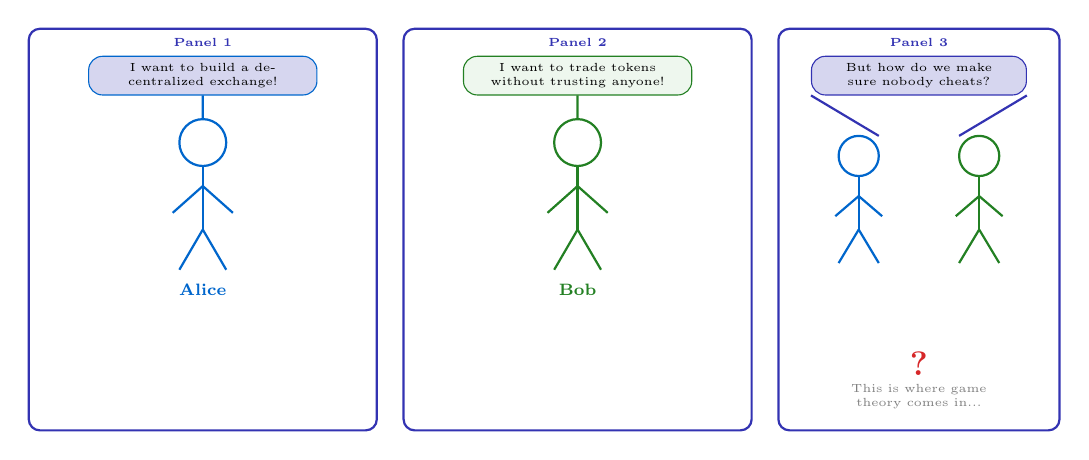
\begin{tikzpicture}[scale=0.85, every node/.style={transform shape}]

% --- Panel 1: Alice ---
\draw[mlpurple, thick, rounded corners=4pt] (-7.2,-2.8) rectangle (-2.0,3.2);
\node[font=\tiny\bfseries, mlpurple] at (-4.6,3.0) {Panel 1};

% Alice stick figure
\draw[mlblue, thick] (-4.6,1.5) circle (0.35);
\draw[mlblue, thick] (-4.6,1.15) -- (-4.6,0.2);
\draw[mlblue, thick] (-4.6,0.85) -- (-5.05,0.45);
\draw[mlblue, thick] (-4.6,0.85) -- (-4.15,0.45);
\draw[mlblue, thick] (-4.6,0.2) -- (-4.95,-0.4);
\draw[mlblue, thick] (-4.6,0.2) -- (-4.25,-0.4);
\node[font=\scriptsize\bfseries, mlblue] at (-4.6,-0.7) {Alice};

% Speech bubble
\node[draw=mlblue, fill=mllavender4, rounded corners=5pt, font=\tiny,
      text width=3.2cm, align=center, inner sep=3pt]
      (alice-bubble) at (-4.6,2.5) {I want to build a decentralized exchange!};
\draw[mlblue, thick] (-4.6,1.85) -- (alice-bubble.south);

% --- Panel 2: Bob ---
\draw[mlpurple, thick, rounded corners=4pt] (-1.6,-2.8) rectangle (3.6,3.2);
\node[font=\tiny\bfseries, mlpurple] at (1.0,3.0) {Panel 2};

% Bob stick figure
\draw[mlgreen!80!black, thick] (1.0,1.5) circle (0.35);
\draw[mlgreen!80!black, thick] (1.0,1.15) -- (1.0,0.2);
\draw[mlgreen!80!black, thick] (1.0,0.85) -- (0.55,0.45);
\draw[mlgreen!80!black, thick] (1.0,0.85) -- (1.45,0.45);
\draw[mlgreen!80!black, thick] (1.0,0.2) -- (0.65,-0.4);
\draw[mlgreen!80!black, thick] (1.0,0.2) -- (1.35,-0.4);
\node[font=\scriptsize\bfseries, mlgreen!80!black] at (1.0,-0.7) {Bob};

% Speech bubble
\node[draw=mlgreen!80!black, fill=mlgreen!8, rounded corners=5pt, font=\tiny,
      text width=3.2cm, align=center, inner sep=3pt]
      (bob-bubble) at (1.0,2.5) {I want to trade tokens without trusting anyone!};
\draw[mlgreen!80!black, thick] (1.0,1.85) -- (bob-bubble.south);

% --- Panel 3: Together ---
\draw[mlpurple, thick, rounded corners=4pt] (4.0,-2.8) rectangle (8.2,3.2);
\node[font=\tiny\bfseries, mlpurple] at (6.1,3.0) {Panel 3};

% Alice (smaller)
\draw[mlblue, thick] (5.2,1.3) circle (0.3);
\draw[mlblue, thick] (5.2,1.0) -- (5.2,0.2);
\draw[mlblue, thick] (5.2,0.7) -- (4.85,0.4);
\draw[mlblue, thick] (5.2,0.7) -- (5.55,0.4);
\draw[mlblue, thick] (5.2,0.2) -- (4.9,-0.3);
\draw[mlblue, thick] (5.2,0.2) -- (5.5,-0.3);

% Bob (smaller)
\draw[mlgreen!80!black, thick] (7.0,1.3) circle (0.3);
\draw[mlgreen!80!black, thick] (7.0,1.0) -- (7.0,0.2);
\draw[mlgreen!80!black, thick] (7.0,0.7) -- (6.65,0.4);
\draw[mlgreen!80!black, thick] (7.0,0.7) -- (7.35,0.4);
\draw[mlgreen!80!black, thick] (7.0,0.2) -- (6.7,-0.3);
\draw[mlgreen!80!black, thick] (7.0,0.2) -- (7.3,-0.3);

% Joint speech bubble
\node[draw=mlpurple, fill=mllavender4, rounded corners=5pt, font=\tiny,
      text width=3.0cm, align=center, inner sep=3pt]
      (joint-bubble) at (6.1,2.5) {But how do we make sure nobody cheats?};
\draw[mlpurple, thick] (5.5,1.6) -- (joint-bubble.south west);
\draw[mlpurple, thick] (6.7,1.6) -- (joint-bubble.south east);

% Question mark
\node[font=\Large\bfseries, mlred] at (6.1,-1.8) {?};
\node[font=\tiny, mlgray, text width=3.5cm, align=center] at (6.1,-2.3) {This is where game theory comes in...};

\end{tikzpicture}
\end{center}
\bottomnote{Every interaction between people with different goals is a `game' --- game theory studies how rational players make decisions.}
\end{frame}

%% ============================================================
%% FRAME 3: JOHN VON NEUMANN — THE FATHER OF GAME THEORY
%% ============================================================
\begin{frame}{John von Neumann --- The Father of Game Theory}
\vspace{-2mm}
\begin{center}
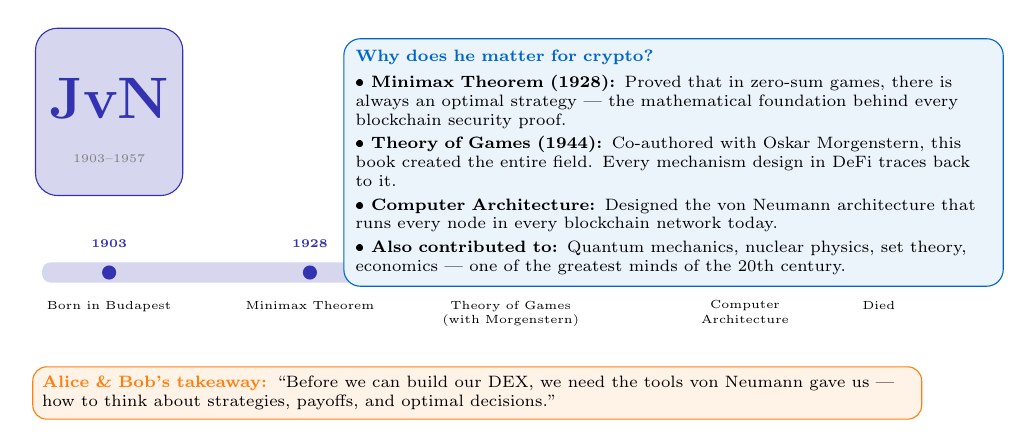
\begin{tikzpicture}[scale=0.85, every node/.style={transform shape}]
% Timeline bar
\fill[mllavender4, rounded corners=3pt] (-6.5,-0.15) rectangle (6.5,0.15);
% Timeline events
\foreach \x/\yr/\lbl in {
  -5.5/1903/Born in Budapest,
  -2.5/1928/Minimax Theorem,
  0.5/1944/\parbox{2.2cm}{\centering Theory of Games\\(with Morgenstern)},
  4.0/1945/\parbox{2.2cm}{\centering Computer\\Architecture},
  6.0/1957/Died}{
  \fill[mlpurple] (\x,0) circle (3pt);
  \node[above, font=\tiny\bfseries, text=mlpurple] at (\x,0.25) {\yr};
  \node[below, font=\tiny, text width=2.2cm, align=center] at (\x,-0.3) {\lbl};
}
% Portrait placeholder — stylized initial
\node[draw=mlpurple, fill=mllavender4, rounded corners=8pt, minimum width=2.2cm, minimum height=2.5cm] at (-5.5, 2.4) {};
\node[font=\Huge\bfseries, text=mlpurple] at (-5.5, 2.6) {JvN};
\node[font=\tiny, text=mlgray] at (-5.5, 1.7) {1903--1957};
% Key contributions panel
\node[draw=mlblue, fill=mlblue!8, rounded corners=6pt, text width=9.5cm, inner sep=5pt, font=\scriptsize, anchor=north west] at (-2.0, 3.5) {%
\textbf{\color{mlblue}Why does he matter for crypto?}\\[3pt]
\textbullet~\textbf{Minimax Theorem (1928):} Proved that in zero-sum games, there is always an optimal strategy --- the mathematical foundation behind every blockchain security proof.\\[2pt]
\textbullet~\textbf{Theory of Games (1944):} Co-authored with Oskar Morgenstern, this book created the entire field. Every mechanism design in DeFi traces back to it.\\[2pt]
\textbullet~\textbf{Computer Architecture:} Designed the von Neumann architecture that runs every node in every blockchain network today.\\[2pt]
\textbullet~\textbf{Also contributed to:} Quantum mechanics, nuclear physics, set theory, economics --- one of the greatest minds of the 20th century.
};
% Connection to Alice & Bob
\node[draw=mlorange, fill=mlorange!10, rounded corners=5pt, font=\scriptsize, inner sep=4pt, text width=13cm] at (0, -1.8) {%
\textbf{\color{mlorange}Alice \& Bob's takeaway:} ``Before we can build our DEX, we need the tools von Neumann gave us --- how to think about strategies, payoffs, and optimal decisions.''
};
\end{tikzpicture}
\end{center}
\bottomnote{John von Neumann proved the Minimax Theorem in 1928 --- the idea that rational players can always find an optimal strategy. This single insight underpins all of blockchain mechanism design.}
\end{frame}

%% ============================================================
%% FRAME 4: WHAT IS GAME THEORY?
%% ============================================================
\begin{frame}{What Is Game Theory?}
\vspace{-2mm}
\begin{center}
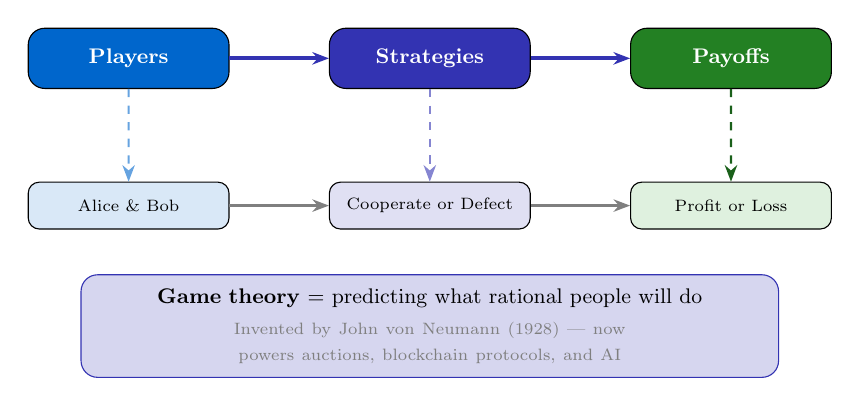
\begin{tikzpicture}[scale=0.85, every node/.style={transform shape}]

% Top row: abstract concepts
\node[gnode=mlblue] (players) at (-4.5,2) {Players};
\node[gnode=mlpurple] (strategies) at (0,2) {Strategies};
\node[gnode=mlgreen!80!black] (payoffs) at (4.5,2) {Payoffs};

\draw[-{Stealth[length=6pt]}, thick, mlpurple, line width=1.5pt] (players) -- (strategies);
\draw[-{Stealth[length=6pt]}, thick, mlpurple, line width=1.5pt] (strategies) -- (payoffs);

% Bottom row: crypto examples
\node[enode=mlblue!15] (ex1) at (-4.5,-0.2) {Alice \& Bob};
\node[enode=mlpurple!15] (ex2) at (0,-0.2) {Cooperate or Defect};
\node[enode=mlgreen!15] (ex3) at (4.5,-0.2) {Profit or Loss};

\draw[-{Stealth[length=6pt]}, thick, mlblue!60, dashed] (players) -- (ex1);
\draw[-{Stealth[length=6pt]}, thick, mlpurple!60, dashed] (strategies) -- (ex2);
\draw[-{Stealth[length=6pt]}, thick, mlgreen!60!black, dashed] (payoffs) -- (ex3);

\draw[-{Stealth[length=6pt]}, thick, mlgray] (ex1) -- (ex2);
\draw[-{Stealth[length=6pt]}, thick, mlgray] (ex2) -- (ex3);

% Key insight box
\node[draw=mlpurple, fill=mllavender4, rounded corners=6pt, font=\small,
      text width=10cm, align=center, inner sep=6pt] at (0,-2.0)
      {\textbf{Game theory} = predicting what rational people will do\\[2pt]
       \textcolor{mlgray}{\scriptsize Invented by John von Neumann (1928) --- now powers auctions, blockchain protocols, and AI}};

\end{tikzpicture}
\end{center}
\bottomnote{Game theory was invented by John von Neumann in 1928 --- it now powers everything from auctions to blockchain protocols.}
\end{frame}

%% ============================================================
%% FRAME 4: THE TRUST DILEMMA
%% ============================================================
\begin{frame}{The Trust Dilemma --- Prisoner's Dilemma}
\vspace{-2mm}
\begin{center}
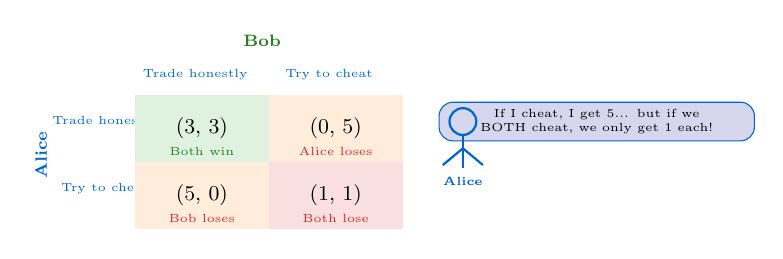
\begin{tikzpicture}[scale=0.85, every node/.style={transform shape}]
  % Header labels
  \node[font=\scriptsize\bfseries, mlgreen!80!black] at (2.5,3.2) {Bob};
  \node[font=\scriptsize\bfseries, mlblue, rotate=90] at (-0.8,1.5) {Alice};
  % Column headers
  \node[font=\tiny, text=mlblue] at (1.5,2.7) {Trade honestly};
  \node[font=\tiny, text=mlblue] at (3.5,2.7) {Try to cheat};
  % Row headers
  \node[font=\tiny, text=mlblue] at (0.15,2) {Trade honestly};
  \node[font=\tiny, text=mlblue] at (0.15,1) {Try to cheat};
  % Grid
  \draw[mlgray] (0.6,0.4) grid[step=2cm] (4.6,2.4);
  % Cells
  \fill[mlgreen!15] (0.6,1.4) rectangle (2.6,2.4);
  \fill[mlorange!15] (2.6,1.4) rectangle (4.6,2.4);
  \fill[mlorange!15] (0.6,0.4) rectangle (2.6,1.4);
  \fill[mlred!15] (2.6,0.4) rectangle (4.6,1.4);
  % Payoff values
  \node[font=\small] at (1.6,1.9) {(3, 3)};
  \node[font=\small] at (3.6,1.9) {(0, 5)};
  \node[font=\small] at (1.6,0.9) {(5, 0)};
  \node[font=\small] at (3.6,0.9) {(1, 1)};

  % Labels
  \node[font=\tiny, mlgreen!80!black] at (1.6,1.55) {Both win};
  \node[font=\tiny, mlred] at (3.6,1.55) {Alice loses};
  \node[font=\tiny, mlred] at (1.6,0.55) {Bob loses};
  \node[font=\tiny, mlred] at (3.6,0.55) {Both lose};

  % Alice speech bubble
  \node[draw=mlblue, fill=mllavender4, rounded corners=5pt, font=\tiny,
        text width=4.5cm, align=center, inner sep=3pt] at (7.5,2.0)
        {If I cheat, I get 5... but if we BOTH cheat, we only get 1 each!};

  % Alice mini figure
  \draw[mlblue, thick] (5.5,2.0) circle (0.2);
  \draw[mlblue, thick] (5.5,1.8) -- (5.5,1.3);
  \draw[mlblue, thick] (5.5,1.6) -- (5.2,1.35);
  \draw[mlblue, thick] (5.5,1.6) -- (5.8,1.35);
  \node[font=\tiny\bfseries, mlblue] at (5.5,1.1) {Alice};

\end{tikzpicture}
\end{center}
\bottomnote{This is the Prisoner's Dilemma --- the most famous game in history. Both players are tempted to cheat, but mutual cooperation gives the best combined outcome.}
\end{frame}

%% ============================================================
%% FRAME 5: JOHN NASH — A BEAUTIFUL MIND
%% ============================================================
\begin{frame}{John Nash --- A Beautiful Mind}
\vspace{-2mm}
\begin{center}
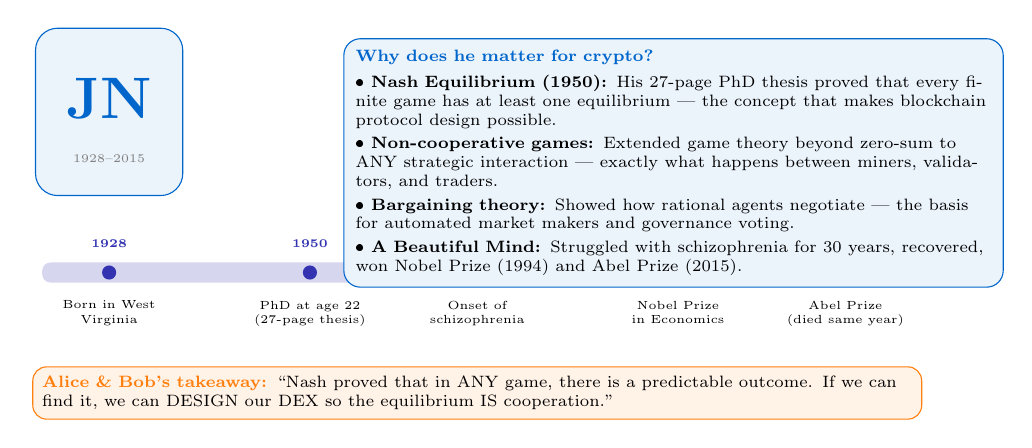
\begin{tikzpicture}[scale=0.85, every node/.style={transform shape}]
% Timeline bar
\fill[mllavender4, rounded corners=3pt] (-6.5,-0.15) rectangle (6.5,0.15);
% Timeline events
\foreach \x/\yr/\lbl in {
  -5.5/1928/Born in West Virginia,
  -2.5/1950/\parbox{2.2cm}{\centering PhD at age 22\\(27-page thesis)},
  0.0/1959/\parbox{2.2cm}{\centering Onset of\\schizophrenia},
  3.0/1994/\parbox{2.2cm}{\centering Nobel Prize\\in Economics},
  5.5/2015/\parbox{2.2cm}{\centering Abel Prize\\(died same year)}}{
  \fill[mlpurple] (\x,0) circle (3pt);
  \node[above, font=\tiny\bfseries, text=mlpurple] at (\x,0.25) {\yr};
  \node[below, font=\tiny, text width=2.2cm, align=center] at (\x,-0.3) {\lbl};
}
% Portrait placeholder
\node[draw=mlblue, fill=mlblue!8, rounded corners=8pt, minimum width=2.2cm, minimum height=2.5cm] at (-5.5, 2.4) {};
\node[font=\Huge\bfseries, text=mlblue] at (-5.5, 2.6) {JN};
\node[font=\tiny, text=mlgray] at (-5.5, 1.7) {1928--2015};
% Key contributions panel
\node[draw=mlblue, fill=mlblue!8, rounded corners=6pt, text width=9.5cm, inner sep=5pt, font=\scriptsize, anchor=north west] at (-2.0, 3.5) {%
\textbf{\color{mlblue}Why does he matter for crypto?}\\[3pt]
\textbullet~\textbf{Nash Equilibrium (1950):} His 27-page PhD thesis proved that every finite game has at least one equilibrium --- the concept that makes blockchain protocol design possible.\\[2pt]
\textbullet~\textbf{Non-cooperative games:} Extended game theory beyond zero-sum to ANY strategic interaction --- exactly what happens between miners, validators, and traders.\\[2pt]
\textbullet~\textbf{Bargaining theory:} Showed how rational agents negotiate --- the basis for automated market makers and governance voting.\\[2pt]
\textbullet~\textbf{A Beautiful Mind:} Struggled with schizophrenia for 30 years, recovered, won Nobel Prize (1994) and Abel Prize (2015).
};
% Connection to Alice & Bob
\node[draw=mlorange, fill=mlorange!10, rounded corners=5pt, font=\scriptsize, inner sep=4pt, text width=13cm] at (0, -1.8) {%
\textbf{\color{mlorange}Alice \& Bob's takeaway:} ``Nash proved that in ANY game, there is a predictable outcome. If we can find it, we can DESIGN our DEX so the equilibrium IS cooperation.''
};
\end{tikzpicture}
\end{center}
\bottomnote{John Nash's 27-page PhD thesis changed the world --- he proved that every finite game has at least one equilibrium, earning him the Nobel Prize 44 years later.}
\end{frame}

%% ============================================================
%% FRAME 6: NASH'S PROOF — EVERY GAME HAS AN EQUILIBRIUM
%% ============================================================
\begin{frame}{Nash's Key Insight --- Every Game Has an Equilibrium}
\vspace{-2mm}
\begin{center}
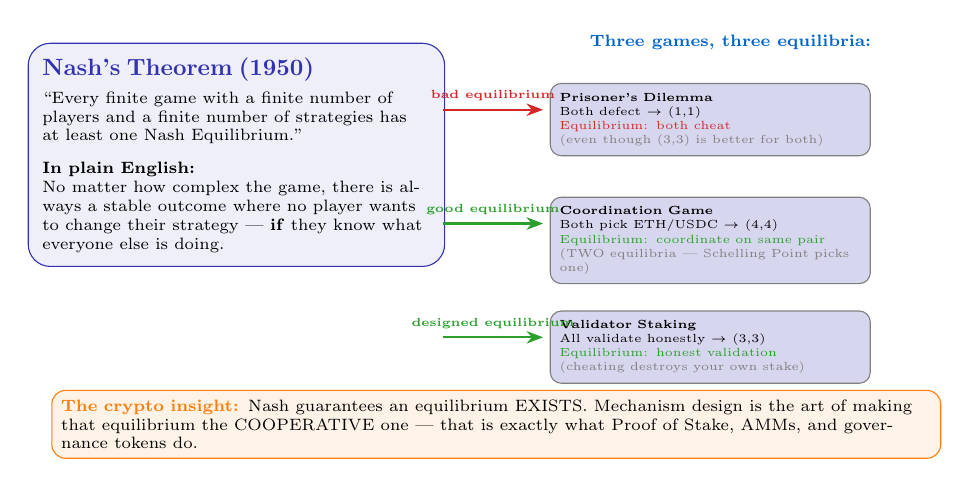
\begin{tikzpicture}[scale=0.85, every node/.style={transform shape}]
% Left: The theorem box
\node[draw=mlpurple, fill=mlpurple!8, rounded corners=8pt, text width=5.8cm, inner sep=6pt, font=\scriptsize, anchor=north west] (theorem) at (-7, 3.2) {%
\textbf{\color{mlpurple}\normalsize Nash's Theorem (1950)}\\[4pt]
``Every finite game with a finite number of players and a finite number of strategies has at least one Nash Equilibrium.''\\[6pt]
\textbf{In plain English:}\\
No matter how complex the game, there is always a stable outcome where no player wants to change their strategy --- \textbf{if} they know what everyone else is doing.
};
% Right: Visual example — 3 games, each with equilibrium marked
\node[font=\scriptsize\bfseries, text=mlblue] at (3.5, 3.2) {Three games, three equilibria:};
% Game 1: Prisoner's Dilemma
\node[draw=mlgray, fill=mllavender4, rounded corners=4pt, text width=4.5cm, inner sep=4pt, font=\tiny, anchor=north west] (g1) at (0.8, 2.6) {%
\textbf{Prisoner's Dilemma}\\
Both defect $\rightarrow$ (1,1)\\
\textcolor{mlred}{Equilibrium: both cheat}\\
\textcolor{mlgray}{(even though (3,3) is better for both)}
};
% Game 2: Coordination Game
\node[draw=mlgray, fill=mllavender4, rounded corners=4pt, text width=4.5cm, inner sep=4pt, font=\tiny, anchor=north west] (g2) at (0.8, 0.9) {%
\textbf{Coordination Game}\\
Both pick ETH/USDC $\rightarrow$ (4,4)\\
\textcolor{mlgreen}{Equilibrium: coordinate on same pair}\\
\textcolor{mlgray}{(TWO equilibria --- Schelling Point picks one)}
};
% Game 3: Staking Game
\node[draw=mlgray, fill=mllavender4, rounded corners=4pt, text width=4.5cm, inner sep=4pt, font=\tiny, anchor=north west] (g3) at (0.8, -0.8) {%
\textbf{Validator Staking}\\
All validate honestly $\rightarrow$ (3,3)\\
\textcolor{mlgreen}{Equilibrium: honest validation}\\
\textcolor{mlgray}{(cheating destroys your own stake)}
};
% Arrow labels
\draw[-{Stealth[length=6pt]}, thick, mlred] (-0.8, 2.2) -- (0.7, 2.2) node[midway, above, font=\tiny\bfseries] {bad equilibrium};
\draw[-{Stealth[length=6pt]}, thick, mlgreen] (-0.8, 0.5) -- (0.7, 0.5) node[midway, above, font=\tiny\bfseries] {good equilibrium};
\draw[-{Stealth[length=6pt]}, thick, mlgreen] (-0.8, -1.2) -- (0.7, -1.2) node[midway, above, font=\tiny\bfseries] {designed equilibrium};
% Bottom insight
\node[draw=mlorange, fill=mlorange!10, rounded corners=5pt, font=\scriptsize, inner sep=4pt, text width=13cm] at (0, -2.5) {%
\textbf{\color{mlorange}The crypto insight:} Nash guarantees an equilibrium EXISTS. Mechanism design is the art of making that equilibrium the COOPERATIVE one --- that is exactly what Proof of Stake, AMMs, and governance tokens do.
};
\end{tikzpicture}
\end{center}
\bottomnote{Nash's theorem guarantees every game has a stable outcome --- the challenge for crypto protocol designers is engineering the rules so that the stable outcome is also the DESIRABLE one.}
\end{frame}

%% ============================================================
%% FRAME 7: NASH EQUILIBRIUM — THE PREDICTABLE OUTCOME
%% ============================================================
\begin{frame}{Nash Equilibrium --- The Predictable Outcome}
\vspace{-2mm}
\begin{center}
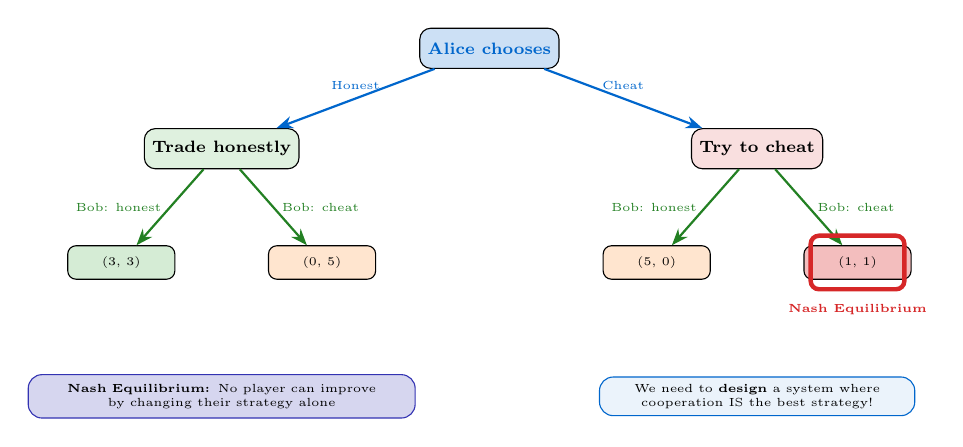
\begin{tikzpicture}[scale=0.85, every node/.style={transform shape}]

% Alice's decision
\node[gtdecision=mlblue!20, text=mlblue] (alice) at (0,3) {Alice chooses};

% Alice branches
\node[gtdecision=mlgreen!15] (a-honest) at (-4,1.5) {Trade honestly};
\node[gtdecision=mlred!15] (a-cheat) at (4,1.5) {Try to cheat};

\draw[-{Stealth[length=6pt]}, thick, mlblue] (alice) -- (a-honest) node[midway, above, font=\tiny] {Honest};
\draw[-{Stealth[length=6pt]}, thick, mlblue] (alice) -- (a-cheat) node[midway, above, font=\tiny] {Cheat};

% Bob's decisions (left branch)
\node[gtoutcome=mlgreen!20] (hh) at (-5.5,-0.2) {(3, 3)};
\node[gtoutcome=mlorange!20] (hc) at (-2.5,-0.2) {(0, 5)};

\draw[-{Stealth[length=6pt]}, thick, mlgreen!80!black] (a-honest) -- (hh) node[midway, left, font=\tiny] {Bob: honest};
\draw[-{Stealth[length=6pt]}, thick, mlgreen!80!black] (a-honest) -- (hc) node[midway, right, font=\tiny] {Bob: cheat};

% Bob's decisions (right branch)
\node[gtoutcome=mlorange!20] (ch) at (2.5,-0.2) {(5, 0)};
\node[gtoutcome=mlred!30] (cc) at (5.5,-0.2) {(1, 1)};

\draw[-{Stealth[length=6pt]}, thick, mlgreen!80!black] (a-cheat) -- (ch) node[midway, left, font=\tiny] {Bob: honest};
\draw[-{Stealth[length=6pt]}, thick, mlgreen!80!black] (a-cheat) -- (cc) node[midway, right, font=\tiny] {Bob: cheat};

% Nash equilibrium highlight
\draw[mlred, ultra thick, rounded corners=3pt] (4.8,-0.6) rectangle (6.2,0.2);
\node[font=\tiny\bfseries, mlred] at (5.5,-0.9) {Nash Equilibrium};

% Explanation box
\node[draw=mlpurple, fill=mllavender4, rounded corners=5pt, font=\tiny,
      text width=5.5cm, align=center, inner sep=4pt] at (-4,-2.2)
      {\textbf{Nash Equilibrium:} No player can improve\\by changing their strategy alone};

% Alice speech bubble
\node[draw=mlblue, fill=mlblue!8, rounded corners=5pt, font=\tiny,
      text width=4.5cm, align=center, inner sep=3pt] at (4,-2.2)
      {We need to \textbf{design} a system where cooperation IS the best strategy!};

\end{tikzpicture}
\end{center}
\bottomnote{John Nash proved every finite game has at least one equilibrium --- the challenge is making the cooperative outcome also be the equilibrium.}
\end{frame}

%% ============================================================
%% FRAME 6: COORDINATION GAME
%% ============================================================
\begin{frame}{The Coordination Game --- Choosing Token Pairs}
\vspace{-2mm}
\begin{center}
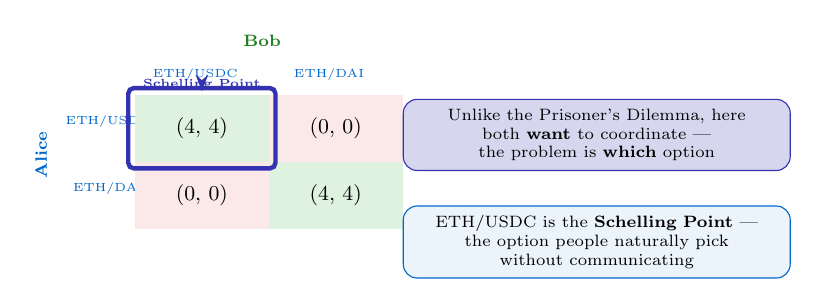
\begin{tikzpicture}[scale=0.85, every node/.style={transform shape}]
  % Header labels
  \node[font=\scriptsize\bfseries, mlgreen!80!black] at (2.5,3.2) {Bob};
  \node[font=\scriptsize\bfseries, mlblue, rotate=90] at (-0.8,1.5) {Alice};
  % Column headers
  \node[font=\tiny, text=mlblue] at (1.5,2.7) {ETH/USDC};
  \node[font=\tiny, text=mlblue] at (3.5,2.7) {ETH/DAI};
  % Row headers
  \node[font=\tiny, text=mlblue] at (0.2,2) {ETH/USDC};
  \node[font=\tiny, text=mlblue] at (0.2,1) {ETH/DAI};
  % Grid
  \draw[mlgray] (0.6,0.4) grid[step=2cm] (4.6,2.4);
  % Cells
  \fill[mlgreen!15] (0.6,1.4) rectangle (2.6,2.4);
  \fill[mlred!10] (2.6,1.4) rectangle (4.6,2.4);
  \fill[mlred!10] (0.6,0.4) rectangle (2.6,1.4);
  \fill[mlgreen!15] (2.6,0.4) rectangle (4.6,1.4);
  % Payoff values
  \node[font=\small] at (1.6,1.9) {(4, 4)};
  \node[font=\small] at (3.6,1.9) {(0, 0)};
  \node[font=\small] at (1.6,0.9) {(0, 0)};
  \node[font=\small] at (3.6,0.9) {(4, 4)};

  % Schelling point highlight
  \draw[mlpurple, ultra thick, rounded corners=2pt] (0.5,1.3) rectangle (2.7,2.5);
  \node[font=\tiny\bfseries, mlpurple] at (1.6,2.55) {Schelling Point};
  \draw[-{Stealth[length=6pt]}, thick, mlpurple] (1.6,2.5) -- (1.6,2.45);

  % Key insight box
  \node[draw=mlpurple, fill=mllavender4, rounded corners=5pt, font=\scriptsize,
        text width=5.5cm, align=center, inner sep=4pt] at (7.5,1.8)
        {Unlike the Prisoner's Dilemma, here\\both \textbf{want} to coordinate ---\\the problem is \textbf{which} option};

  % Second insight
  \node[draw=mlblue, fill=mlblue!8, rounded corners=5pt, font=\scriptsize,
        text width=5.5cm, align=center, inner sep=4pt] at (7.5,0.2)
        {ETH/USDC is the \textbf{Schelling Point} ---\\the option people naturally pick\\without communicating};

\end{tikzpicture}
\end{center}
\bottomnote{A Schelling Point is the option people naturally converge on without communicating --- in crypto, ETH is almost always the Schelling Point for trading pairs.}
\end{frame}

%% ============================================================
%% FRAME 6b: COORDINATION GAME — DEEP DIVE
%% ============================================================
\begin{frame}{Coordination Games --- Why They Matter in Crypto}
\vspace{-3mm}
\begin{center}
\adjustbox{max width=\textwidth,max totalheight=6.5cm}{%
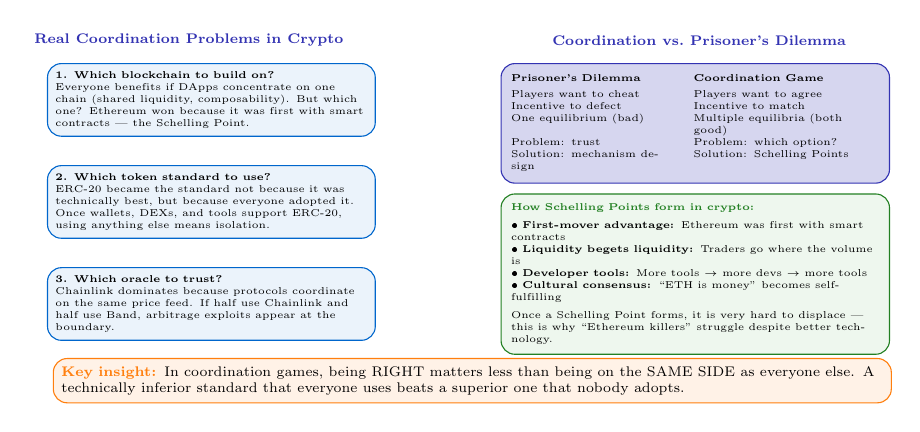
\begin{tikzpicture}[scale=0.72, every node/.style={transform shape}]
% Left column: Real crypto coordination examples
\node[font=\scriptsize\bfseries, text=mlpurple] at (-5, 4.2) {Real Coordination Problems in Crypto};

\node[draw=mlblue, fill=mlblue!8, rounded corners=5pt, text width=5.5cm, inner sep=4pt, font=\tiny, anchor=north west] (ex1) at (-7.5, 3.8) {%
\textbf{1. Which blockchain to build on?}\\
Everyone benefits if DApps concentrate on one chain (shared liquidity, composability). But which one? Ethereum won because it was first with smart contracts --- the Schelling Point.
};

\node[draw=mlblue, fill=mlblue!8, rounded corners=5pt, text width=5.5cm, inner sep=4pt, font=\tiny, anchor=north west] (ex2) at (-7.5, 2.0) {%
\textbf{2. Which token standard to use?}\\
ERC-20 became the standard not because it was technically best, but because everyone adopted it. Once wallets, DEXs, and tools support ERC-20, using anything else means isolation.
};

\node[draw=mlblue, fill=mlblue!8, rounded corners=5pt, text width=5.5cm, inner sep=4pt, font=\tiny, anchor=north west] (ex3) at (-7.5, 0.2) {%
\textbf{3. Which oracle to trust?}\\
Chainlink dominates because protocols coordinate on the same price feed. If half use Chainlink and half use Band, arbitrage exploits appear at the boundary.
};

% Right column: Key differences from Prisoner's Dilemma
\node[font=\scriptsize\bfseries, text=mlpurple] at (4, 4.2) {Coordination vs.\ Prisoner's Dilemma};

% Comparison table
\node[draw=mlpurple, fill=mllavender4, rounded corners=5pt, text width=6.5cm, inner sep=5pt, font=\tiny, anchor=north west] at (0.5, 3.8) {%
\begin{tabular}{@{}p{2.8cm}p{3.0cm}@{}}
\textbf{Prisoner's Dilemma} & \textbf{Coordination Game} \\[2pt]
Players want to cheat & Players want to agree \\
Incentive to defect & Incentive to match \\
One equilibrium (bad) & Multiple equilibria (both good) \\
Problem: trust & Problem: which option? \\
Solution: mechanism design & Solution: Schelling Points \\
\end{tabular}
};

% How Schelling Points form
\node[draw=mlgreen!80!black, fill=mlgreen!8, rounded corners=5pt, text width=6.5cm, inner sep=5pt, font=\tiny, anchor=north west] at (0.5, 1.5) {%
\textbf{\color{mlgreen!80!black}How Schelling Points form in crypto:}\\[3pt]
\textbullet~\textbf{First-mover advantage:} Ethereum was first with smart contracts\\
\textbullet~\textbf{Liquidity begets liquidity:} Traders go where the volume is\\
\textbullet~\textbf{Developer tools:} More tools $\rightarrow$ more devs $\rightarrow$ more tools\\
\textbullet~\textbf{Cultural consensus:} ``ETH is money'' becomes self-fulfilling\\[3pt]
Once a Schelling Point forms, it is very hard to displace --- this is why ``Ethereum killers'' struggle despite better technology.
};

% Bottom insight
\node[draw=mlorange, fill=mlorange!10, rounded corners=5pt, font=\scriptsize, inner sep=4pt, text width=14.5cm] at (0, -1.8) {%
\textbf{\color{mlorange}Key insight:} In coordination games, being RIGHT matters less than being on the SAME SIDE as everyone else. A technically inferior standard that everyone uses beats a superior one that nobody adopts.
};
\end{tikzpicture}%
}%
\end{center}
\bottomnote{Coordination games explain why crypto has ``winner-take-most'' dynamics --- once a standard or platform becomes the Schelling Point, network effects make it nearly impossible to displace.}
\end{frame}

%% ============================================================
%% FRAME 7: FREE RIDER PROBLEM
%% ============================================================
\begin{frame}{Who Provides Liquidity? --- The Free Rider Problem}
\vspace{-2mm}
\begin{center}
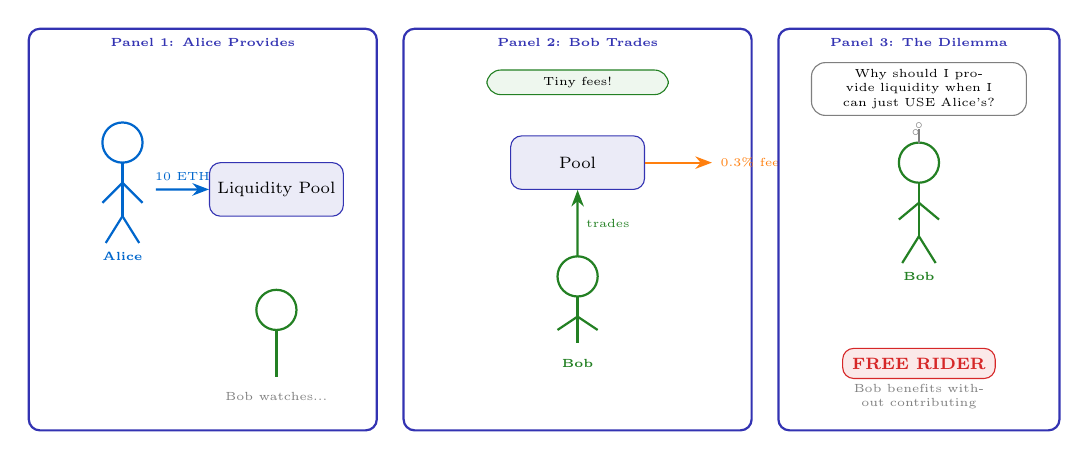
\begin{tikzpicture}[scale=0.85, every node/.style={transform shape}]

% --- Panel 1: Alice provides liquidity ---
\draw[mlpurple, thick, rounded corners=4pt] (-7.2,-2.8) rectangle (-2.0,3.2);
\node[font=\tiny\bfseries, mlpurple] at (-4.6,3.0) {Panel 1: Alice Provides};

% Alice stick figure
\draw[mlblue, thick] (-5.8,1.5) circle (0.3);
\draw[mlblue, thick] (-5.8,1.2) -- (-5.8,0.4);
\draw[mlblue, thick] (-5.8,0.9) -- (-6.1,0.6);
\draw[mlblue, thick] (-5.8,0.9) -- (-5.5,0.6);
\draw[mlblue, thick] (-5.8,0.4) -- (-6.05,0.0);
\draw[mlblue, thick] (-5.8,0.4) -- (-5.55,0.0);
\node[font=\tiny\bfseries, mlblue] at (-5.8,-0.2) {Alice};

% Pool box
\node[draw=mlpurple, fill=mlpurple!10, rounded corners=4pt, font=\scriptsize,
      minimum width=2cm, minimum height=0.8cm] (pool1) at (-3.5,0.8) {Liquidity Pool};
\draw[-{Stealth[length=6pt]}, thick, mlblue] (-5.3,0.8) -- (pool1.west)
      node[midway, above, font=\tiny] {10 ETH};

% Bob watching
\draw[mlgreen!80!black, thick] (-3.5,-1.0) circle (0.3);
\draw[mlgreen!80!black, thick] (-3.5,-1.3) -- (-3.5,-2.0);
\node[font=\tiny, mlgray] at (-3.5,-2.3) {Bob watches...};

% --- Panel 2: Bob trades ---
\draw[mlpurple, thick, rounded corners=4pt] (-1.6,-2.8) rectangle (3.6,3.2);
\node[font=\tiny\bfseries, mlpurple] at (1.0,3.0) {Panel 2: Bob Trades};

% Pool
\node[draw=mlpurple, fill=mlpurple!10, rounded corners=4pt, font=\scriptsize,
      minimum width=2cm, minimum height=0.8cm] (pool2) at (1.0,1.2) {Pool};

% Bob
\draw[mlgreen!80!black, thick] (1.0,-0.5) circle (0.3);
\draw[mlgreen!80!black, thick] (1.0,-0.8) -- (1.0,-1.5);
\draw[mlgreen!80!black, thick] (1.0,-1.1) -- (0.7,-1.3);
\draw[mlgreen!80!black, thick] (1.0,-1.1) -- (1.3,-1.3);
\node[font=\tiny\bfseries, mlgreen!80!black] at (1.0,-1.8) {Bob};

\draw[-{Stealth[length=6pt]}, thick, mlgreen!80!black] (1.0,-0.2) -- (pool2.south)
      node[midway, right, font=\tiny] {trades};

% Fee arrow
\draw[-{Stealth[length=6pt]}, thick, mlorange] (pool2.east) -- ++(1.0,0)
      node[right, font=\tiny] {0.3\% fee};

% Speech bubble
\node[draw=mlgreen!80!black, fill=mlgreen!8, rounded corners=5pt, font=\tiny,
      text width=2.5cm, align=center, inner sep=3pt] at (1.0,2.4) {Tiny fees!};

% --- Panel 3: Bob's dilemma ---
\draw[mlpurple, thick, rounded corners=4pt] (4.0,-2.8) rectangle (8.2,3.2);
\node[font=\tiny\bfseries, mlpurple] at (6.1,3.0) {Panel 3: The Dilemma};

% Bob thinking
\draw[mlgreen!80!black, thick] (6.1,1.2) circle (0.3);
\draw[mlgreen!80!black, thick] (6.1,0.9) -- (6.1,0.1);
\draw[mlgreen!80!black, thick] (6.1,0.6) -- (5.8,0.35);
\draw[mlgreen!80!black, thick] (6.1,0.6) -- (6.4,0.35);
\draw[mlgreen!80!black, thick] (6.1,0.1) -- (5.85,-0.3);
\draw[mlgreen!80!black, thick] (6.1,0.1) -- (6.35,-0.3);
\node[font=\tiny\bfseries, mlgreen!80!black] at (6.1,-0.5) {Bob};

% Thought bubble
\node[draw=mlgray, fill=white, rounded corners=5pt, font=\tiny,
      text width=3.0cm, align=center, inner sep=3pt] at (6.1,2.3)
      {Why should I provide liquidity when I can just USE Alice's?};
\draw[mlgray] (6.1,1.5) -- (6.1,1.7);
\node[font=\tiny, mlgray] at (6.05,1.65) {$\circ$};
\node[font=\tiny, mlgray] at (6.1,1.75) {$\circ$};

% FREE RIDER label
\node[draw=mlred, fill=mlred!10, rounded corners=4pt, font=\scriptsize\bfseries,
      text=mlred, inner sep=4pt] at (6.1,-1.8) {FREE RIDER};
\node[font=\tiny, mlgray, text width=3cm, align=center] at (6.1,-2.3)
      {Bob benefits without contributing};

\end{tikzpicture}
\end{center}
\bottomnote{The Free Rider Problem occurs when individuals benefit from a public good without paying for it --- Uniswap solved this with liquidity mining rewards.}
\end{frame}

%% ============================================================
%% FRAME 8: MECHANISM DESIGN
%% ============================================================
\begin{frame}{Mechanism Design --- Incentivizing Cooperation}
\vspace{-2mm}
\begin{center}
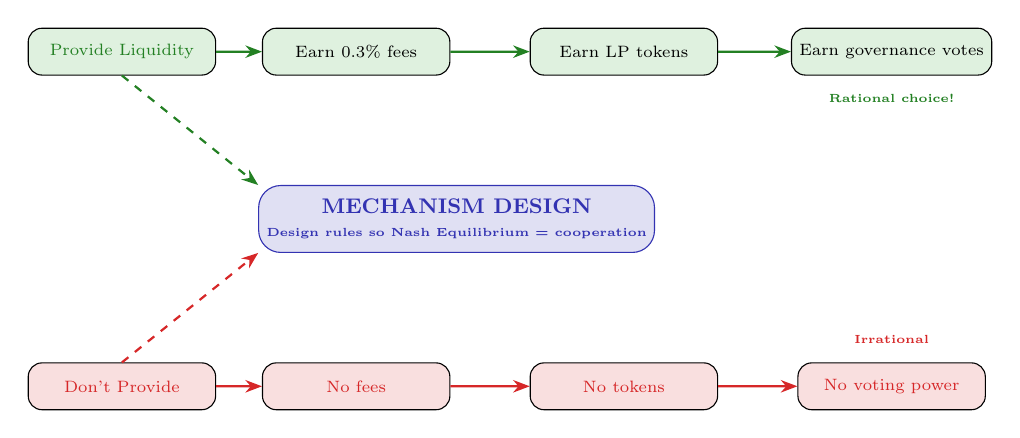
\begin{tikzpicture}[scale=0.85, every node/.style={transform shape}]

% Central concept
\node[draw=mlpurple, fill=mlpurple!15, rounded corners=8pt, font=\small\bfseries,
      text=mlpurple, minimum width=5cm, minimum height=1cm, align=center]
      (center) at (0,0.5) {MECHANISM DESIGN\\[-1pt]\tiny Design rules so Nash Equilibrium = cooperation};

% Provide path (left/top)
\node[mbox=mlgreen!15, text=mlgreen!80!black] (provide) at (-5,3) {Provide Liquidity};
\node[mbox=mlgreen!15] (fees) at (-1.5,3) {Earn 0.3\% fees};
\node[mbox=mlgreen!15] (lp) at (2.5,3) {Earn LP tokens};
\node[mbox=mlgreen!15] (gov) at (6.5,3) {Earn governance votes};

\draw[-{Stealth[length=6pt]}, thick, mlgreen!80!black] (provide) -- (fees);
\draw[-{Stealth[length=6pt]}, thick, mlgreen!80!black] (fees) -- (lp);
\draw[-{Stealth[length=6pt]}, thick, mlgreen!80!black] (lp) -- (gov);

% Don't provide path (right/bottom)
\node[mbox=mlred!15, text=mlred] (noprovide) at (-5,-2) {Don't Provide};
\node[mbox=mlred!15, text=mlred] (nofees) at (-1.5,-2) {No fees};
\node[mbox=mlred!15, text=mlred] (notokens) at (2.5,-2) {No tokens};
\node[mbox=mlred!15, text=mlred] (novotes) at (6.5,-2) {No voting power};

\draw[-{Stealth[length=6pt]}, thick, mlred] (noprovide) -- (nofees);
\draw[-{Stealth[length=6pt]}, thick, mlred] (nofees) -- (notokens);
\draw[-{Stealth[length=6pt]}, thick, mlred] (notokens) -- (novotes);

% Connecting arrows to center
\draw[-{Stealth[length=6pt]}, thick, mlgreen!80!black, dashed] (provide.south) -- (center.north west);
\draw[-{Stealth[length=6pt]}, thick, mlred, dashed] (noprovide.north) -- (center.south west);

% Result labels
\node[font=\tiny\bfseries, mlgreen!80!black] at (6.5,2.3) {Rational choice!};
\node[font=\tiny\bfseries, mlred] at (6.5,-1.3) {Irrational};

\end{tikzpicture}
\end{center}
\bottomnote{Mechanism design is `reverse game theory' --- instead of predicting behavior, you design the rules so the desired behavior becomes the rational choice.}
\end{frame}

%% ============================================================
%% FRAME 9: AMM PRICE DISCOVERY (dense)
%% ============================================================
\begin{frame}{The Price Discovery Game --- How AMMs Work}
\vspace{-3mm}
\begin{center}
\adjustbox{max width=\textwidth,max totalheight=6.5cm}{%
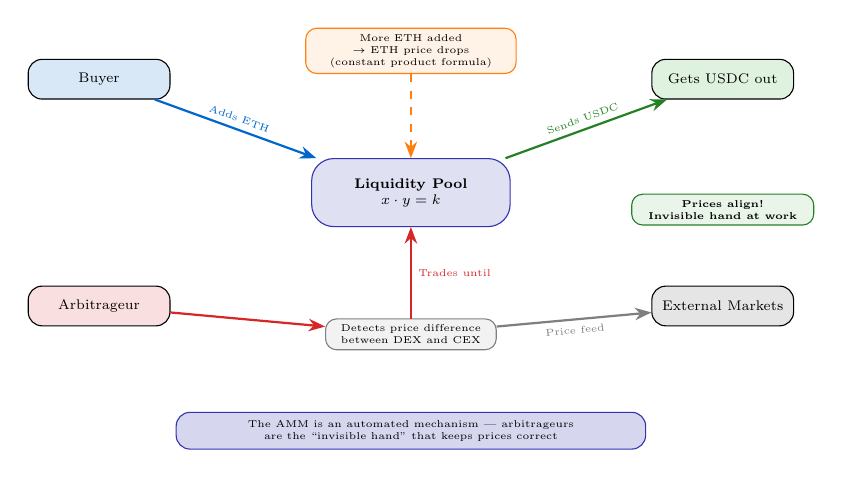
\begin{tikzpicture}[scale=0.72, every node/.style={transform shape}]

% Central pool
\node[pool] (pool) at (0,0) {Liquidity Pool\\$x \cdot y = k$};

% Buyer
\node[actor=mlblue!15] (buyer) at (-5.5,2) {Buyer};
\draw[-{Stealth[length=6pt]}, thick, mlblue] (buyer) -- (pool)
      node[midway, above, sloped, font=\tiny] {Adds ETH};

% Seller output
\node[actor=mlgreen!15] (output) at (5.5,2) {Gets USDC out};
\draw[-{Stealth[length=6pt]}, thick, mlgreen!80!black] (pool) -- (output)
      node[midway, above, sloped, font=\tiny] {Sends USDC};

% Price impact
\node[draw=mlorange, fill=mlorange!10, rounded corners=4pt, font=\tiny,
      text width=3.5cm, align=center, inner sep=3pt] (price) at (0,2.5)
      {More ETH added $\rightarrow$ ETH price drops\\(constant product formula)};
\draw[-{Stealth[length=6pt]}, thick, mlorange, dashed] (price) -- (pool);

% Arbitrageur
\node[actor=mlred!15] (arb) at (-5.5,-2) {Arbitrageur};
\node[draw=mlgray, fill=mlgray!10, rounded corners=4pt, font=\tiny,
      text width=2.8cm, align=center, inner sep=3pt] (detect) at (0,-2.5)
      {Detects price difference\\between DEX and CEX};
\draw[-{Stealth[length=6pt]}, thick, mlred] (arb) -- (detect);
\draw[-{Stealth[length=6pt]}, thick, mlred] (detect) -- (pool)
      node[midway, right, font=\tiny] {Trades until};

% External market
\node[actor=mlgray!20] (market) at (5.5,-2) {External Markets};
\draw[{Stealth[length=6pt]}-, thick, mlgray] (market) -- (detect)
      node[midway, below, sloped, font=\tiny] {Price feed};

% Result arrow
\node[draw=mlgreen!80!black, fill=mlgreen!10, rounded corners=4pt, font=\tiny\bfseries,
      text width=3cm, align=center, inner sep=3pt] at (5.5,-0.3)
      {Prices align!\\Invisible hand at work};

% Key insight
\node[draw=mlpurple, fill=mllavender4, rounded corners=5pt, font=\tiny,
      text width=8cm, align=center, inner sep=4pt] at (0,-4.2)
      {The AMM is an automated mechanism --- arbitrageurs are the ``invisible hand'' that keeps prices correct};

\end{tikzpicture}%
}%
\end{center}
\bottomnote{Automated Market Makers replace traditional order books with a mathematical formula --- game theory ensures arbitrageurs keep prices aligned with the market.}
\end{frame}

%% ============================================================
%% FRAME 9b: AMM DEEP DIVE — THE GAME THEORY BEHIND PRICE DISCOVERY
%% ============================================================
\begin{frame}{How AMMs Really Work --- The Game Behind the Formula}
\vspace{-3mm}
\begin{center}
\adjustbox{max width=\textwidth,max totalheight=6.5cm}{%
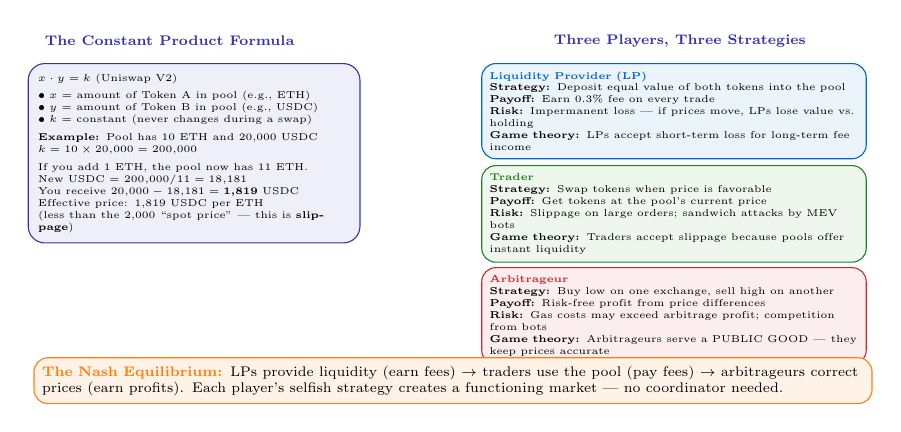
\begin{tikzpicture}[scale=0.72, every node/.style={transform shape}]
% Column 1: The constant product formula explained
\node[font=\scriptsize\bfseries, text=mlpurple] at (-5, 4.2) {The Constant Product Formula};

\node[draw=mlpurple, fill=mlpurple!8, rounded corners=6pt, text width=5.5cm, inner sep=5pt, font=\tiny, anchor=north west] at (-7.5, 3.8) {%
\textbf{$x \cdot y = k$} (Uniswap V2)\\[3pt]
\textbullet~$x$ = amount of Token A in pool (e.g., ETH)\\
\textbullet~$y$ = amount of Token B in pool (e.g., USDC)\\
\textbullet~$k$ = constant (never changes during a swap)\\[3pt]
\textbf{Example:} Pool has 10 ETH and 20{,}000 USDC\\
$k = 10 \times 20{,}000 = 200{,}000$\\[3pt]
If you add 1 ETH, the pool now has 11 ETH.\\
New USDC = $200{,}000 / 11 = 18{,}181$\\
You receive $20{,}000 - 18{,}181 = \textbf{1{,}819}$ USDC\\
Effective price: 1{,}819 USDC per ETH\\
(less than the 2{,}000 ``spot price'' --- this is \textbf{slippage})
};

% Column 2: The three-player game
\node[font=\scriptsize\bfseries, text=mlpurple] at (4, 4.2) {Three Players, Three Strategies};

% Player 1: Liquidity Provider
\node[draw=mlblue, fill=mlblue!8, rounded corners=5pt, text width=6.5cm, inner sep=4pt, font=\tiny, anchor=north west] at (0.5, 3.8) {%
\textbf{\color{mlblue}Liquidity Provider (LP)}\\
\textbf{Strategy:} Deposit equal value of both tokens into the pool\\
\textbf{Payoff:} Earn 0.3\% fee on every trade\\
\textbf{Risk:} Impermanent loss --- if prices move, LPs lose value vs.\ holding\\
\textbf{Game theory:} LPs accept short-term loss for long-term fee income
};

% Player 2: Trader
\node[draw=mlgreen!80!black, fill=mlgreen!8, rounded corners=5pt, text width=6.5cm, inner sep=4pt, font=\tiny, anchor=north west] at (0.5, 2.0) {%
\textbf{\color{mlgreen!80!black}Trader}\\
\textbf{Strategy:} Swap tokens when price is favorable\\
\textbf{Payoff:} Get tokens at the pool's current price\\
\textbf{Risk:} Slippage on large orders; sandwich attacks by MEV bots\\
\textbf{Game theory:} Traders accept slippage because pools offer instant liquidity
};

% Player 3: Arbitrageur
\node[draw=mlred, fill=mlred!8, rounded corners=5pt, text width=6.5cm, inner sep=4pt, font=\tiny, anchor=north west] at (0.5, 0.2) {%
\textbf{\color{mlred}Arbitrageur}\\
\textbf{Strategy:} Buy low on one exchange, sell high on another\\
\textbf{Payoff:} Risk-free profit from price differences\\
\textbf{Risk:} Gas costs may exceed arbitrage profit; competition from bots\\
\textbf{Game theory:} Arbitrageurs serve a PUBLIC GOOD --- they keep prices accurate
};

% Bottom: Why this works
\node[draw=mlorange, fill=mlorange!10, rounded corners=5pt, font=\scriptsize, inner sep=4pt, text width=14.5cm] at (0, -1.8) {%
\textbf{\color{mlorange}The Nash Equilibrium:} LPs provide liquidity (earn fees) $\rightarrow$ traders use the pool (pay fees) $\rightarrow$ arbitrageurs correct prices (earn profits). Each player's selfish strategy creates a functioning market --- no coordinator needed.
};
\end{tikzpicture}%
}%
\end{center}
\bottomnote{AMMs are a triumph of mechanism design --- three types of selfish players (LPs, traders, arbitrageurs) each pursuing profit, yet together they create a fair, efficient, 24/7 market.}
\end{frame}

%% ============================================================
%% FRAME 10: VALIDATOR'S DILEMMA
%% ============================================================
\begin{frame}{The Validator's Dilemma}
\vspace{-2mm}
\begin{center}
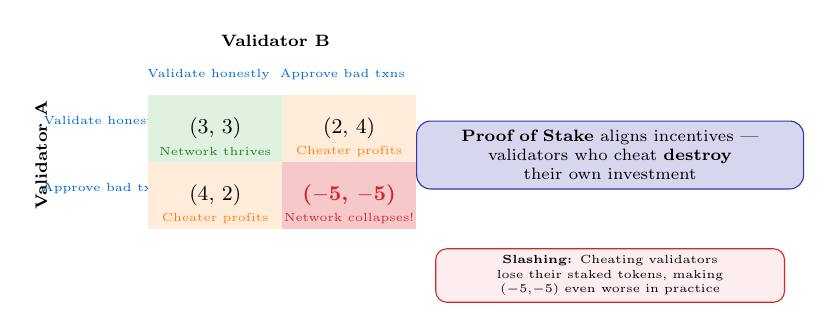
\begin{tikzpicture}[scale=0.85, every node/.style={transform shape}]
  % Header labels
  \node[font=\scriptsize\bfseries] at (2.5,3.2) {Validator B};
  \node[font=\scriptsize\bfseries, rotate=90] at (-1.0,1.5) {Validator A};
  % Column headers
  \node[font=\tiny, text=mlblue] at (1.5,2.7) {Validate honestly};
  \node[font=\tiny, text=mlblue] at (3.5,2.7) {Approve bad txns};
  % Row headers
  \node[font=\tiny, text=mlblue] at (-0.05,2) {Validate honestly};
  \node[font=\tiny, text=mlblue] at (-0.05,1) {Approve bad txns};
  % Grid
  \draw[mlgray] (0.6,0.4) grid[step=2cm] (4.6,2.4);
  % Cells
  \fill[mlgreen!15] (0.6,1.4) rectangle (2.6,2.4);
  \fill[mlorange!15] (2.6,1.4) rectangle (4.6,2.4);
  \fill[mlorange!15] (0.6,0.4) rectangle (2.6,1.4);
  \fill[mlred!25] (2.6,0.4) rectangle (4.6,1.4);
  % Payoff values
  \node[font=\small] at (1.6,1.9) {(3, 3)};
  \node[font=\small] at (3.6,1.9) {(2, 4)};
  \node[font=\small] at (1.6,0.9) {(4, 2)};
  \node[font=\small\bfseries, mlred] at (3.6,0.9) {($-$5, $-$5)};

  % Labels
  \node[font=\tiny, mlgreen!80!black] at (1.6,1.55) {Network thrives};
  \node[font=\tiny, mlorange] at (3.6,1.55) {Cheater profits};
  \node[font=\tiny, mlorange] at (1.6,0.55) {Cheater profits};
  \node[font=\tiny, mlred] at (3.6,0.55) {Network collapses!};

  % Key insight box
  \node[draw=mlpurple, fill=mllavender4, rounded corners=5pt, font=\scriptsize,
        text width=5.5cm, align=center, inner sep=4pt] at (7.5,1.5)
        {\textbf{Proof of Stake} aligns incentives ---\\validators who cheat \textbf{destroy}\\their own investment};

  % Slashing note
  \node[draw=mlred, fill=mlred!8, rounded corners=4pt, font=\tiny,
        text width=5cm, align=center, inner sep=3pt] at (7.5,-0.3)
        {\textbf{Slashing:} Cheating validators lose their staked tokens,
         making ($-$5,$-$5) even worse in practice};

\end{tikzpicture}
\end{center}
\bottomnote{This is why validators must `stake' tokens --- it makes honest behavior the dominant strategy because cheating destroys your own wealth.}
\end{frame}

%% ============================================================
%% FRAME 10b: VALIDATOR'S DILEMMA — DEEP DIVE
%% ============================================================
\begin{frame}{The Validator's Dilemma --- Why Proof of Stake Works}
\vspace{-3mm}
\begin{center}
\adjustbox{max width=\textwidth,max totalheight=6.5cm}{%
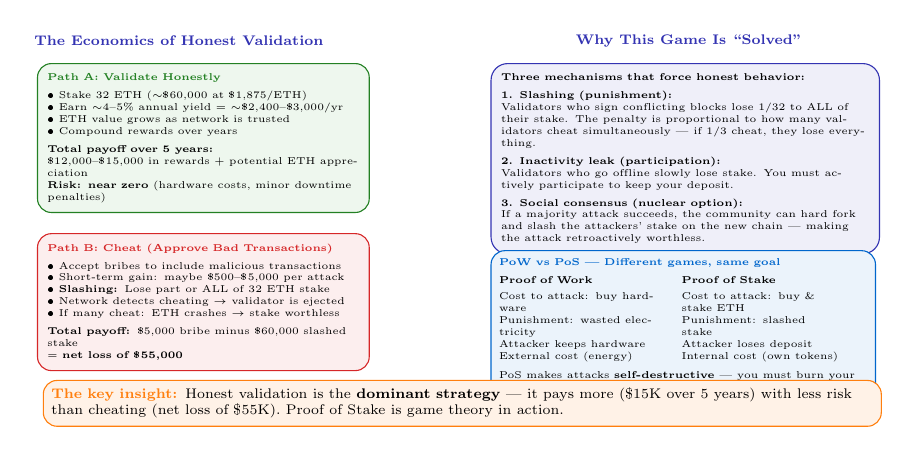
\begin{tikzpicture}[scale=0.72, every node/.style={transform shape}]
% Left: The economics of honest validation
\node[font=\scriptsize\bfseries, text=mlpurple] at (-5, 4.2) {The Economics of Honest Validation};

\node[draw=mlgreen!80!black, fill=mlgreen!8, rounded corners=5pt, text width=5.5cm, inner sep=5pt, font=\tiny, anchor=north west] at (-7.5, 3.8) {%
\textbf{\color{mlgreen!80!black}Path A: Validate Honestly}\\[3pt]
\textbullet~Stake 32 ETH ($\sim$\$60{,}000 at \$1{,}875/ETH)\\
\textbullet~Earn $\sim$4--5\% annual yield = $\sim$\$2{,}400--\$3{,}000/yr\\
\textbullet~ETH value grows as network is trusted\\
\textbullet~Compound rewards over years\\[3pt]
\textbf{Total payoff over 5 years:}\\
\$12{,}000--\$15{,}000 in rewards + potential ETH appreciation\\
\textbf{Risk: near zero} (hardware costs, minor downtime penalties)
};

\node[draw=mlred, fill=mlred!8, rounded corners=5pt, text width=5.5cm, inner sep=5pt, font=\tiny, anchor=north west] at (-7.5, 0.8) {%
\textbf{\color{mlred}Path B: Cheat (Approve Bad Transactions)}\\[3pt]
\textbullet~Accept bribes to include malicious transactions\\
\textbullet~Short-term gain: maybe \$500--\$5{,}000 per attack\\
\textbullet~\textbf{Slashing:} Lose part or ALL of 32 ETH stake\\
\textbullet~Network detects cheating $\rightarrow$ validator is ejected\\
\textbullet~If many cheat: ETH crashes $\rightarrow$ stake worthless\\[3pt]
\textbf{Total payoff:} \$5{,}000 bribe minus \$60{,}000 slashed stake\\
= \textbf{net loss of \$55{,}000}
};

% Right: Why this is a solved game
\node[font=\scriptsize\bfseries, text=mlpurple] at (4, 4.2) {Why This Game Is ``Solved''};

\node[draw=mlpurple, fill=mlpurple!8, rounded corners=6pt, text width=6.5cm, inner sep=5pt, font=\tiny, anchor=north west] at (0.5, 3.8) {%
\textbf{Three mechanisms that force honest behavior:}\\[3pt]
\textbf{1. Slashing (punishment):}\\
Validators who sign conflicting blocks lose 1/32 to ALL of their stake. The penalty is proportional to how many validators cheat simultaneously --- if 1/3 cheat, they lose everything.\\[3pt]
\textbf{2. Inactivity leak (participation):}\\
Validators who go offline slowly lose stake. You must actively participate to keep your deposit.\\[3pt]
\textbf{3. Social consensus (nuclear option):}\\
If a majority attack succeeds, the community can hard fork and slash the attackers' stake on the new chain --- making the attack retroactively worthless.
};

% Comparison: PoW vs PoS incentives
\node[draw=mlblue, fill=mlblue!8, rounded corners=5pt, text width=6.5cm, inner sep=4pt, font=\tiny, anchor=north west] at (0.5, 0.5) {%
\textbf{\color{mlblue}PoW vs PoS --- Different games, same goal}\\[3pt]
\begin{tabular}{@{}p{2.8cm}p{2.8cm}@{}}
\textbf{Proof of Work} & \textbf{Proof of Stake} \\[2pt]
Cost to attack: buy hardware & Cost to attack: buy \& stake ETH \\
Punishment: wasted electricity & Punishment: slashed stake \\
Attacker keeps hardware & Attacker loses deposit \\
External cost (energy) & Internal cost (own tokens) \\
\end{tabular}\\[3pt]
PoS makes attacks \textbf{self-destructive} --- you must burn your own wealth to attack, then your attack devalues that wealth further.
};

% Bottom insight
\node[draw=mlorange, fill=mlorange!10, rounded corners=5pt, font=\scriptsize, inner sep=4pt, text width=14.5cm] at (0, -2.2) {%
\textbf{\color{mlorange}The key insight:} Honest validation is the \textbf{dominant strategy} --- it pays more (\$15K over 5 years) with less risk than cheating (net loss of \$55K). Proof of Stake is game theory in action.
};
\end{tikzpicture}%
}%
\end{center}
\bottomnote{Proof of Stake turns blockchain security into a game theory problem with a clear solution: staking makes honesty profitable and cheating financially suicidal.}
\end{frame}

%% ============================================================
%% FRAME 11: SKIN IN THE GAME
%% ============================================================
\begin{frame}{Skin in the Game --- Why Staking Works}
\vspace{-2mm}
\begin{center}
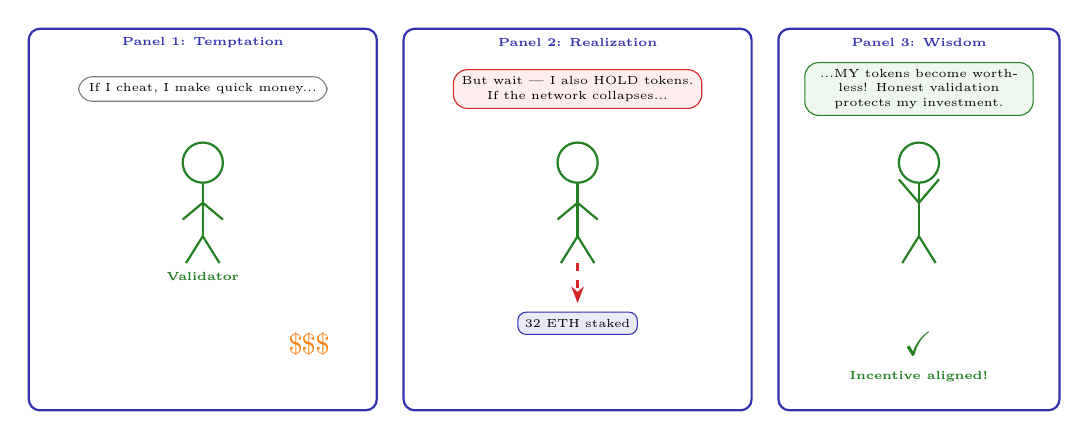
\begin{tikzpicture}[scale=0.85, every node/.style={transform shape}]

% --- Panel 1: Temptation ---
\draw[mlpurple, thick, rounded corners=4pt] (-7.2,-2.5) rectangle (-2.0,3.2);
\node[font=\tiny\bfseries, mlpurple] at (-4.6,3.0) {Panel 1: Temptation};

% Validator stick figure
\draw[mlgreen!80!black, thick] (-4.6,1.2) circle (0.3);
\draw[mlgreen!80!black, thick] (-4.6,0.9) -- (-4.6,0.1);
\draw[mlgreen!80!black, thick] (-4.6,0.6) -- (-4.9,0.35);
\draw[mlgreen!80!black, thick] (-4.6,0.6) -- (-4.3,0.35);
\draw[mlgreen!80!black, thick] (-4.6,0.1) -- (-4.85,-0.3);
\draw[mlgreen!80!black, thick] (-4.6,0.1) -- (-4.35,-0.3);
\node[font=\tiny\bfseries, mlgreen!80!black] at (-4.6,-0.5) {Validator};

% Thought bubble
\node[draw=mlgray, fill=white, rounded corners=5pt, font=\tiny,
      text width=3.5cm, align=center, inner sep=3pt] at (-4.6,2.3)
      {If I cheat, I make quick money...};

% Money symbol
\node[font=\large, mlorange] at (-3.0,-1.5) {\$\$\$};

% --- Panel 2: Realization ---
\draw[mlpurple, thick, rounded corners=4pt] (-1.6,-2.5) rectangle (3.6,3.2);
\node[font=\tiny\bfseries, mlpurple] at (1.0,3.0) {Panel 2: Realization};

% Same validator
\draw[mlgreen!80!black, thick] (1.0,1.2) circle (0.3);
\draw[mlgreen!80!black, thick] (1.0,0.9) -- (1.0,0.1);
\draw[mlgreen!80!black, thick] (1.0,0.6) -- (0.7,0.35);
\draw[mlgreen!80!black, thick] (1.0,0.6) -- (1.3,0.35);
\draw[mlgreen!80!black, thick] (1.0,0.1) -- (0.75,-0.3);
\draw[mlgreen!80!black, thick] (1.0,0.1) -- (1.25,-0.3);

% Thought bubble
\node[draw=mlred, fill=mlred!8, rounded corners=5pt, font=\tiny,
      text width=3.5cm, align=center, inner sep=3pt] at (1.0,2.3)
      {But wait --- I also HOLD tokens. If the network collapses...};

% Token stack
\node[draw=mlpurple, fill=mlpurple!10, rounded corners=3pt, font=\tiny,
      inner sep=3pt] at (1.0,-1.2) {32 ETH staked};
\draw[-{Stealth[length=6pt]}, thick, mlred, dashed] (1.0,-0.3) -- (1.0,-0.9);

% --- Panel 3: Wisdom ---
\draw[mlpurple, thick, rounded corners=4pt] (4.0,-2.5) rectangle (8.2,3.2);
\node[font=\tiny\bfseries, mlpurple] at (6.1,3.0) {Panel 3: Wisdom};

% Happy validator
\draw[mlgreen!80!black, thick] (6.1,1.2) circle (0.3);
\draw[mlgreen!80!black, thick] (6.1,0.9) -- (6.1,0.1);
\draw[mlgreen!80!black, thick] (6.1,0.6) -- (5.8,0.95);
\draw[mlgreen!80!black, thick] (6.1,0.6) -- (6.4,0.95);
\draw[mlgreen!80!black, thick] (6.1,0.1) -- (5.85,-0.3);
\draw[mlgreen!80!black, thick] (6.1,0.1) -- (6.35,-0.3);

% Speech bubble
\node[draw=mlgreen!80!black, fill=mlgreen!8, rounded corners=5pt, font=\tiny,
      text width=3.2cm, align=center, inner sep=3pt] at (6.1,2.3)
      {...MY tokens become worthless! Honest validation protects my investment.};

% Checkmark
\node[font=\Large, mlgreen!80!black] at (6.1,-1.5) {\checkmark};
\node[font=\tiny\bfseries, mlgreen!80!black] at (6.1,-2.0) {Incentive aligned!};

\end{tikzpicture}
\end{center}
\bottomnote{Staking creates `skin in the game' --- validators who cheat destroy their own wealth, so honest behavior is the rational choice.}
\end{frame}

%% ============================================================
%% FRAME 12: SIGNALING
%% ============================================================
\begin{frame}{Signaling --- How to Spot Good Projects}
\vspace{-2mm}
\begin{center}
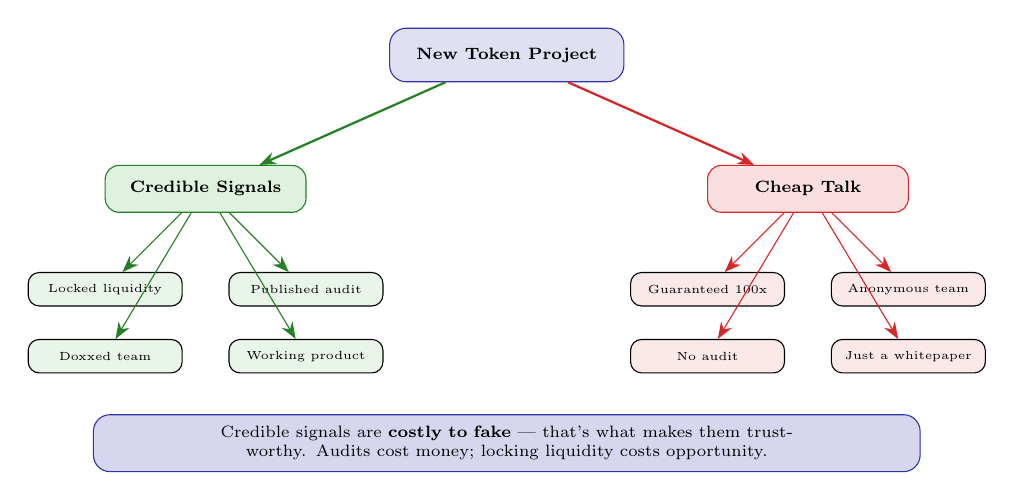
\begin{tikzpicture}[scale=0.85, every node/.style={transform shape}]

% Root node
\node[draw=mlpurple, fill=mlpurple!15, rounded corners=6pt, font=\scriptsize\bfseries,
      minimum width=3.5cm, minimum height=0.8cm] (root) at (0,3) {New Token Project};

% Branches
\node[draw=mlgreen!80!black, fill=mlgreen!15, rounded corners=5pt, font=\scriptsize\bfseries,
      minimum width=3cm, minimum height=0.7cm] (credible) at (-4.5,1) {Credible Signals};
\node[draw=mlred, fill=mlred!15, rounded corners=5pt, font=\scriptsize\bfseries,
      minimum width=3cm, minimum height=0.7cm] (cheap) at (4.5,1) {Cheap Talk};

\draw[-{Stealth[length=6pt]}, thick, mlgreen!80!black] (root) -- (credible);
\draw[-{Stealth[length=6pt]}, thick, mlred] (root) -- (cheap);

% Credible signals
\node[sig=mlgreen!10] (s1) at (-6,-0.5) {Locked liquidity};
\node[sig=mlgreen!10] (s2) at (-3,-0.5) {Published audit};
\node[sig=mlgreen!10] (s3) at (-6,-1.5) {Doxxed team};
\node[sig=mlgreen!10] (s4) at (-3,-1.5) {Working product};

\draw[-{Stealth[length=6pt]}, mlgreen!80!black] (credible) -- (s1);
\draw[-{Stealth[length=6pt]}, mlgreen!80!black] (credible) -- (s2);
\draw[-{Stealth[length=6pt]}, mlgreen!80!black] (credible) -- (s3);
\draw[-{Stealth[length=6pt]}, mlgreen!80!black] (credible) -- (s4);

% Cheap talk
\node[sig=mlred!10] (c1) at (3,-0.5) {Guaranteed 100x};
\node[sig=mlred!10] (c2) at (6,-0.5) {Anonymous team};
\node[sig=mlred!10] (c3) at (3,-1.5) {No audit};
\node[sig=mlred!10] (c4) at (6,-1.5) {Just a whitepaper};

\draw[-{Stealth[length=6pt]}, mlred] (cheap) -- (c1);
\draw[-{Stealth[length=6pt]}, mlred] (cheap) -- (c2);
\draw[-{Stealth[length=6pt]}, mlred] (cheap) -- (c3);
\draw[-{Stealth[length=6pt]}, mlred] (cheap) -- (c4);

% Key insight
\node[draw=mlpurple, fill=mllavender4, rounded corners=6pt, font=\scriptsize,
      text width=12cm, align=center, inner sep=5pt] at (0,-2.8)
      {Credible signals are \textbf{costly to fake} --- that's what makes them trustworthy.
       Audits cost money; locking liquidity costs opportunity.};

\end{tikzpicture}
\end{center}
\bottomnote{In game theory, a credible signal is one that is expensive to produce if you're lying --- audits cost money, locking liquidity costs opportunity.}
\end{frame}

%% ============================================================
%% FRAME 13: SCHELLING POINTS & NETWORK EFFECTS
%% ============================================================
\begin{frame}{Why Everyone Uses ETH --- Schelling Points \& Network Effects}
\vspace{-2mm}
\begin{center}
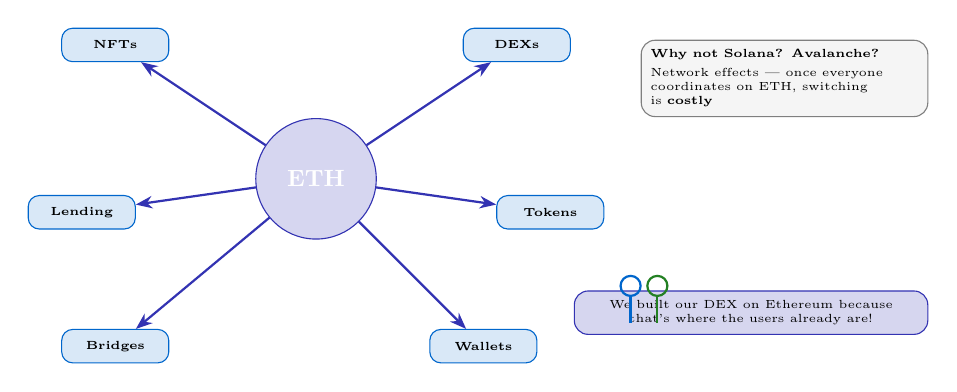
\begin{tikzpicture}[scale=0.85, every node/.style={transform shape}]

% Central ETH hub
\node[draw=mlpurple, fill=mlpurple!20, circle, font=\normalsize\bfseries,
      minimum size=1.8cm, text=white] (eth) at (0,0.5) {ETH};

% Surrounding nodes
\node[draw=mlblue, fill=mlblue!15, rounded corners=4pt, font=\tiny\bfseries,
      minimum width=1.6cm, minimum height=0.5cm] (dex) at (3,2.5) {DEXs};
\node[draw=mlblue, fill=mlblue!15, rounded corners=4pt, font=\tiny\bfseries,
      minimum width=1.6cm, minimum height=0.5cm] (tokens) at (3.5,0) {Tokens};
\node[draw=mlblue, fill=mlblue!15, rounded corners=4pt, font=\tiny\bfseries,
      minimum width=1.6cm, minimum height=0.5cm] (wallets) at (2.5,-2) {Wallets};
\node[draw=mlblue, fill=mlblue!15, rounded corners=4pt, font=\tiny\bfseries,
      minimum width=1.6cm, minimum height=0.5cm] (bridges) at (-3,-2) {Bridges};
\node[draw=mlblue, fill=mlblue!15, rounded corners=4pt, font=\tiny\bfseries,
      minimum width=1.6cm, minimum height=0.5cm] (lending) at (-3.5,0) {Lending};
\node[draw=mlblue, fill=mlblue!15, rounded corners=4pt, font=\tiny\bfseries,
      minimum width=1.6cm, minimum height=0.5cm] (nfts) at (-3,2.5) {NFTs};

% Connections
\draw[-{Stealth[length=6pt]}, thick, mlpurple] (eth) -- (dex);
\draw[-{Stealth[length=6pt]}, thick, mlpurple] (eth) -- (tokens);
\draw[-{Stealth[length=6pt]}, thick, mlpurple] (eth) -- (wallets);
\draw[-{Stealth[length=6pt]}, thick, mlpurple] (eth) -- (bridges);
\draw[-{Stealth[length=6pt]}, thick, mlpurple] (eth) -- (lending);
\draw[-{Stealth[length=6pt]}, thick, mlpurple] (eth) -- (nfts);

% Comparison box
\node[draw=mlgray, fill=mlgray!8, rounded corners=5pt, font=\tiny,
      text width=4cm, align=left, inner sep=4pt] at (7,2)
      {\textbf{Why not Solana? Avalanche?}\\[2pt]
       Network effects --- once everyone\\coordinates on ETH, switching\\is \textbf{costly}};

% Alice & Bob bubble
\node[draw=mlpurple, fill=mllavender4, rounded corners=5pt, font=\tiny,
      text width=5cm, align=center, inner sep=4pt] at (6.5,-1.5)
      {We built our DEX on Ethereum because\\that's where the users already are!};

% Mini figures
\draw[mlblue, thick] (4.7,-1.1) circle (0.15);
\draw[mlblue, thick] (4.7,-1.25) -- (4.7,-1.65);
\draw[mlgreen!80!black, thick] (5.1,-1.1) circle (0.15);
\draw[mlgreen!80!black, thick] (5.1,-1.25) -- (5.1,-1.65);

\end{tikzpicture}
\end{center}
\bottomnote{Network effects create powerful Schelling Points --- the more people use a platform, the more valuable it becomes, making it the rational default choice.}
\end{frame}

%% ============================================================
%% FRAME 13b: SCHELLING POINTS & NETWORK EFFECTS — DEEP DIVE
%% ============================================================
\begin{frame}{Network Effects --- The Flywheel That Cannot Be Stopped}
\vspace{-3mm}
\begin{center}
\adjustbox{max width=\textwidth,max totalheight=6.5cm}{%
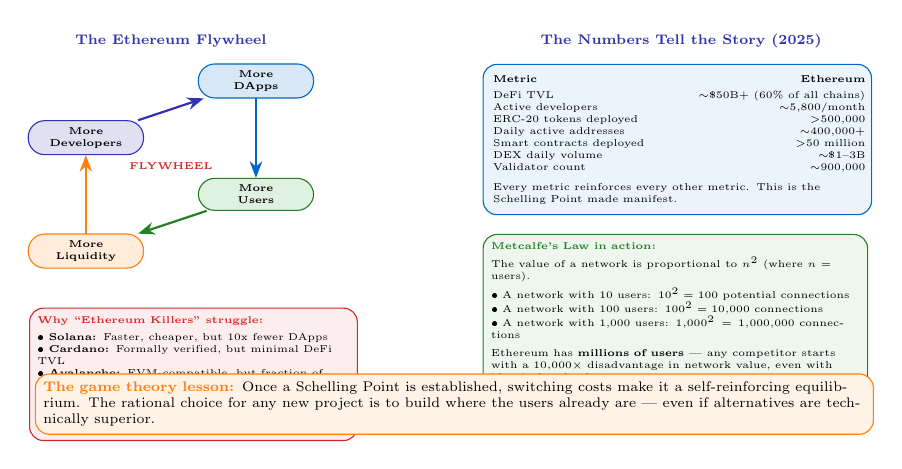
\begin{tikzpicture}[scale=0.72, every node/.style={transform shape}]
% Left: The network effect flywheel
\node[font=\scriptsize\bfseries, text=mlpurple] at (-5, 4.2) {The Ethereum Flywheel};

% Circular flywheel
\node[draw=mlpurple, fill=mlpurple!15, rounded corners=6pt, font=\tiny\bfseries, text width=1.8cm, align=center] (devs) at (-6.5, 2.5) {More\\Developers};
\node[draw=mlblue, fill=mlblue!15, rounded corners=6pt, font=\tiny\bfseries, text width=1.8cm, align=center] (apps) at (-3.5, 3.5) {More\\DApps};
\node[draw=mlgreen!80!black, fill=mlgreen!15, rounded corners=6pt, font=\tiny\bfseries, text width=1.8cm, align=center] (users) at (-3.5, 1.5) {More\\Users};
\node[draw=mlorange, fill=mlorange!15, rounded corners=6pt, font=\tiny\bfseries, text width=1.8cm, align=center] (liq) at (-6.5, 0.5) {More\\Liquidity};

\draw[-{Stealth[length=6pt]}, thick, mlpurple] (devs) -- (apps);
\draw[-{Stealth[length=6pt]}, thick, mlblue] (apps) -- (users);
\draw[-{Stealth[length=6pt]}, thick, mlgreen!80!black] (users) -- (liq);
\draw[-{Stealth[length=6pt]}, thick, mlorange] (liq) -- (devs);

\node[font=\tiny\bfseries, text=mlred] at (-5, 2) {FLYWHEEL};

% Why competitors fail
\node[draw=mlred, fill=mlred!8, rounded corners=5pt, text width=5.5cm, inner sep=4pt, font=\tiny, anchor=north west] at (-7.5, -0.5) {%
\textbf{\color{mlred}Why ``Ethereum Killers'' struggle:}\\[3pt]
\textbullet~\textbf{Solana:} Faster, cheaper, but 10x fewer DApps\\
\textbullet~\textbf{Cardano:} Formally verified, but minimal DeFi TVL\\
\textbullet~\textbf{Avalanche:} EVM-compatible, but fraction of liquidity\\[3pt]
They can match Ethereum's \textit{technology} but not its \textit{network effects}. The flywheel gives the incumbent an exponentially growing advantage.
};

% Right: Real numbers
\node[font=\scriptsize\bfseries, text=mlpurple] at (4, 4.2) {The Numbers Tell the Story (2025)};

\node[draw=mlblue, fill=mlblue!8, rounded corners=5pt, text width=6.5cm, inner sep=5pt, font=\tiny, anchor=north west] at (0.5, 3.8) {%
\begin{tabular}{@{}p{3.2cm}r@{}}
\textbf{Metric} & \textbf{Ethereum} \\[2pt]
DeFi TVL & $\sim$\$50B+ (60\% of all chains) \\
Active developers & $\sim$5{,}800/month \\
ERC-20 tokens deployed & $>$500{,}000 \\
Daily active addresses & $\sim$400{,}000+ \\
Smart contracts deployed & $>$50 million \\
DEX daily volume & $\sim$\$1--3B \\
Validator count & $\sim$900{,}000 \\
\end{tabular}\\[4pt]
Every metric reinforces every other metric. This is the Schelling Point made manifest.
};

% Metcalfe's Law
\node[draw=mlgreen!80!black, fill=mlgreen!8, rounded corners=5pt, text width=6.5cm, inner sep=4pt, font=\tiny, anchor=north west] at (0.5, 0.8) {%
\textbf{\color{mlgreen!80!black}Metcalfe's Law in action:}\\[3pt]
The value of a network is proportional to $n^2$ (where $n$ = users).\\[2pt]
\textbullet~A network with 10 users: $10^2 = 100$ potential connections\\
\textbullet~A network with 100 users: $100^2 = 10{,}000$ connections\\
\textbullet~A network with 1{,}000 users: $1{,}000^2 = 1{,}000{,}000$ connections\\[3pt]
Ethereum has \textbf{millions of users} --- any competitor starts with a $10{,}000\times$ disadvantage in network value, even with identical technology.
};

% Bottom insight
\node[draw=mlorange, fill=mlorange!10, rounded corners=5pt, font=\scriptsize, inner sep=4pt, text width=14.5cm] at (0, -2.2) {%
\textbf{\color{mlorange}The game theory lesson:} Once a Schelling Point is established, switching costs make it a self-reinforcing equilibrium. The rational choice for any new project is to build where the users already are --- even if alternatives are technically superior.
};
\end{tikzpicture}%
}%
\end{center}
\bottomnote{Metcalfe's Law means network effects grow quadratically --- Ethereum's dominance is not about better technology, it is about having a flywheel that competitors cannot replicate without matching its entire ecosystem.}
\end{frame}

%% ============================================================
%% FRAME 14: THE HAPPY ENDING
%% ============================================================
\begin{frame}{Alice \& Bob's DEX --- Game Theory in Action}
\vspace{-2mm}
\begin{center}
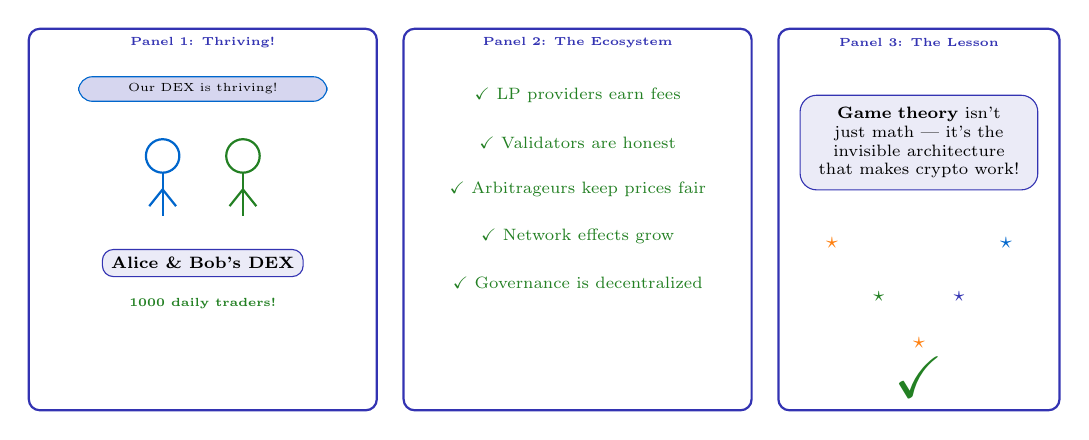
\begin{tikzpicture}[scale=0.85, every node/.style={transform shape}]

% --- Panel 1: Thriving DEX ---
\draw[mlpurple, thick, rounded corners=4pt] (-7.2,-2.5) rectangle (-2.0,3.2);
\node[font=\tiny\bfseries, mlpurple] at (-4.6,3.0) {Panel 1: Thriving!};

% Alice & Bob together
\draw[mlblue, thick] (-5.2,1.3) circle (0.25);
\draw[mlblue, thick] (-5.2,1.05) -- (-5.2,0.4);
\draw[mlblue, thick] (-5.2,0.8) -- (-5.4,0.55);
\draw[mlblue, thick] (-5.2,0.8) -- (-5.0,0.55);
\draw[mlgreen!80!black, thick] (-4.0,1.3) circle (0.25);
\draw[mlgreen!80!black, thick] (-4.0,1.05) -- (-4.0,0.4);
\draw[mlgreen!80!black, thick] (-4.0,0.8) -- (-4.2,0.55);
\draw[mlgreen!80!black, thick] (-4.0,0.8) -- (-3.8,0.55);

% DEX box
\node[draw=mlpurple, fill=mlpurple!10, rounded corners=4pt, font=\scriptsize\bfseries,
      minimum width=3cm] at (-4.6,-0.3) {Alice \& Bob's DEX};
\node[font=\tiny\bfseries, mlgreen!80!black] at (-4.6,-0.9) {1000 daily traders!};

% Speech bubble
\node[draw=mlblue, fill=mllavender4, rounded corners=5pt, font=\tiny,
      text width=3.5cm, align=center, inner sep=3pt] at (-4.6,2.3) {Our DEX is thriving!};

% --- Panel 2: Ecosystem ---
\draw[mlpurple, thick, rounded corners=4pt] (-1.6,-2.5) rectangle (3.6,3.2);
\node[font=\tiny\bfseries, mlpurple] at (1.0,3.0) {Panel 2: The Ecosystem};

% Checkmarks
\node[font=\scriptsize, mlgreen!80!black] at (1.0,2.2) {\checkmark\ LP providers earn fees};
\node[font=\scriptsize, mlgreen!80!black] at (1.0,1.5) {\checkmark\ Validators are honest};
\node[font=\scriptsize, mlgreen!80!black] at (1.0,0.8) {\checkmark\ Arbitrageurs keep prices fair};
\node[font=\scriptsize, mlgreen!80!black] at (1.0,0.1) {\checkmark\ Network effects grow};
\node[font=\scriptsize, mlgreen!80!black] at (1.0,-0.6) {\checkmark\ Governance is decentralized};

% --- Panel 3: Lesson ---
\draw[mlpurple, thick, rounded corners=4pt] (4.0,-2.5) rectangle (8.2,3.2);
\node[font=\tiny\bfseries, mlpurple] at (6.1,3.0) {Panel 3: The Lesson};

% Speech bubble with key message
\node[draw=mlpurple, fill=mlpurple!10, rounded corners=6pt, font=\scriptsize,
      text width=3.2cm, align=center, inner sep=5pt] at (6.1,1.5)
      {\textbf{Game theory} isn't just math --- it's the invisible architecture that makes crypto work!};

% Celebration: stars
\node[font=\normalsize, mlorange] at (4.8,0.0) {$\star$};
\node[font=\normalsize, mlblue] at (7.4,0.0) {$\star$};
\node[font=\small, mlgreen!80!black] at (5.5,-0.8) {$\star$};
\node[font=\small, mlpurple] at (6.7,-0.8) {$\star$};
\node[font=\normalsize, mlorange] at (6.1,-1.5) {$\star$};

% Checkmark
\node[font=\Huge, mlgreen!80!black] at (6.1,-2.0) {\checkmark};

\end{tikzpicture}
\end{center}
\bottomnote{Every DeFi protocol is a carefully designed game --- understanding game theory helps you evaluate which ones will succeed and which will fail.}
\end{frame}

%% ============================================================
%% FRAME 15: KEY TERMS (dense)
%% ============================================================
\begin{frame}{Key Terms for Beginners}
\vspace{-2mm}
\begin{center}
\adjustbox{max width=\textwidth,max totalheight=6.8cm}{%
\scriptsize
\begin{columns}[T]
\begin{column}{0.48\linewidth}
\renewcommand{\arraystretch}{1.15}
\begin{tabular}{@{}>{\columncolor{mllavender4}}p{2.1cm}p{4.4cm}@{}}
\toprule
\textbf{\color{mlpurple}Term} & \textbf{\color{mlpurple}Definition} \\
\midrule
Game Theory & Study of strategic decision-making between rational players \\
\rowcolor{white}
Player & A decision-maker in a game (Alice, Bob, a validator) \\
Strategy & A complete plan of action (cooperate or defect) \\
\rowcolor{white}
Payoff & The reward or penalty from a strategy outcome \\
Nash Equilibrium & No player can improve by changing strategy alone \\
\rowcolor{white}
Dominant Strategy & Best response regardless of what others do \\
Prisoner's Dilemma & Both tempted to defect, but cooperation is better \\
\bottomrule
\end{tabular}
\end{column}
\begin{column}{0.48\linewidth}
\renewcommand{\arraystretch}{1.15}
\begin{tabular}{@{}>{\columncolor{mlblue!8}}p{2.2cm}p{4.3cm}@{}}
\toprule
\textbf{\color{mlblue}Term} & \textbf{\color{mlblue}Definition} \\
\midrule
Coordination Game & Players benefit from choosing the same option \\
\rowcolor{white}
Free Rider & Benefits from a public good without contributing \\
Mechanism Design & Designing rules so desired behavior is rational \\
\rowcolor{white}
Schelling Point & The option people naturally converge on \\
Signaling & Costly actions that reveal private information \\
\rowcolor{white}
Network Effect & More users = more value for everyone \\
AMM & Automated Market Maker --- math replaces order books \\
\bottomrule
\end{tabular}
\end{column}
\end{columns}
}%
\end{center}
\bottomnote{Master these 14 terms and you can analyze any crypto protocol through a game theory lens.}
\end{frame}

%% ============================================================
%% FRAME 16: KEY TAKEAWAYS
%% ============================================================
\begin{frame}{Key Takeaways}
\vspace{-2mm}
\begin{center}
\adjustbox{max width=\textwidth,max totalheight=6.8cm}{%
\scriptsize
\renewcommand{\arraystretch}{1.4}
\begin{tabular}{@{}c >{\raggedright\arraybackslash}p{10.5cm}@{}}
\toprule
\textbf{\color{mlpurple}\#} & \textbf{\color{mlpurple}Takeaway} \\
\midrule
\rowcolor{mlpurple!6}
\textbf{\Large\color{mlpurple}1} & Every crypto interaction is a \textbf{game} with players, strategies, and payoffs --- understanding the game is the first step to understanding the protocol. \\
\textbf{\Large\color{mlblue}2} & The \textbf{Prisoner's Dilemma} explains why trust-free systems need mechanism design --- without it, rational players defect and the system collapses. \\
\rowcolor{mlpurple!6}
\textbf{\Large\color{mlgreen!70!black}3} & \textbf{Proof of Stake} works because validators have skin in the game --- cheating costs more than cooperating (slashing makes honesty the dominant strategy). \\
\textbf{\Large\color{mlorange}4} & \textbf{Schelling Points} and network effects explain why everyone uses ETH --- coordination on a focal point creates a self-reinforcing equilibrium. \\
\rowcolor{mlpurple!6}
\textbf{\Large\color{mlred}5} & Good \textbf{mechanism design} makes cooperation the Nash Equilibrium --- the protocol designer's job is to align individual incentives with collective welfare. \\
\bottomrule
\end{tabular}
}%
\end{center}
\bottomnote{Game theory is the invisible engine behind every successful blockchain protocol.}
\end{frame}

%% ============================================================
%% FRAME 17: APPENDIX SECTION DIVIDER
%% ============================================================
\begin{frame}{}
\vfill
\begin{beamercolorbox}[sep=12pt,center,rounded=true,shadow=true]{palette quaternary}
{\Large\bfseries Appendix: Going Deeper}\\[6pt]
{\normalsize Formal concepts, advanced examples, and further resources}
\end{beamercolorbox}
\vfill
\end{frame}

%% ============================================================
%% FRAME 18: FORMAL PAYOFF MATRICES (dense)
%% ============================================================
\begin{frame}{Formal Payoff Matrices Explained}
\vspace{-3mm}
\begin{center}
\adjustbox{max width=\textwidth,max totalheight=6.5cm}{%
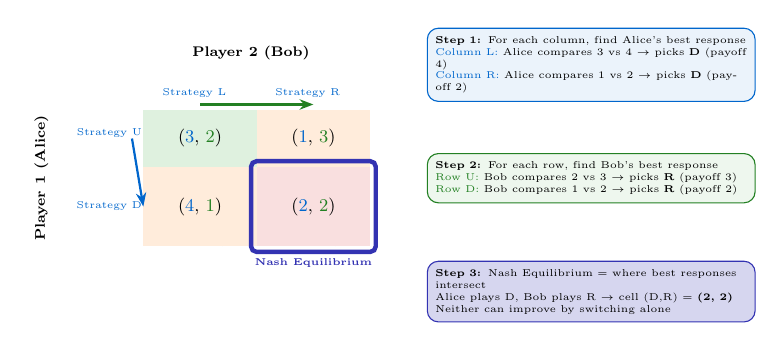
\begin{tikzpicture}[scale=0.72, every node/.style={transform shape}]

  % The matrix
  \node[font=\scriptsize\bfseries] at (2.5,4.2) {Player 2 (Bob)};
  \node[font=\scriptsize\bfseries, rotate=90] at (-1.2,2.0) {Player 1 (Alice)};

  \node[font=\tiny, text=mlblue] at (1.5,3.5) {Strategy L};
  \node[font=\tiny, text=mlblue] at (3.5,3.5) {Strategy R};
  \node[font=\tiny, text=mlblue] at (0.0,2.8) {Strategy U};
  \node[font=\tiny, text=mlblue] at (0.0,1.5) {Strategy D};

  \draw[mlgray, thick] (0.6,0.8) grid[step=2cm] (4.6,3.2);

  \fill[mlgreen!15] (0.6,2.2) rectangle (2.6,3.2);
  \fill[mlorange!15] (2.6,2.2) rectangle (4.6,3.2);
  \fill[mlorange!15] (0.6,0.8) rectangle (2.6,2.2);
  \fill[mlred!15] (2.6,0.8) rectangle (4.6,2.2);

  \node[font=\small] at (1.6,2.7) {(\textcolor{mlblue}{3}, \textcolor{mlgreen!80!black}{2})};
  \node[font=\small] at (3.6,2.7) {(\textcolor{mlblue}{1}, \textcolor{mlgreen!80!black}{3})};
  \node[font=\small] at (1.6,1.5) {(\textcolor{mlblue}{4}, \textcolor{mlgreen!80!black}{1})};
  \node[font=\small] at (3.6,1.5) {(\textcolor{mlblue}{2}, \textcolor{mlgreen!80!black}{2})};

  % Step-by-step annotations
  \node[draw=mlblue, fill=mlblue!8, rounded corners=4pt, font=\tiny,
        text width=5.5cm, inner sep=4pt, align=left] at (8.5,4.0)
        {\textbf{Step 1:} For each column, find Alice's best response\\
         \textcolor{mlblue}{Column L:} Alice compares 3 vs 4 $\rightarrow$ picks \textbf{D} (payoff 4)\\
         \textcolor{mlblue}{Column R:} Alice compares 1 vs 2 $\rightarrow$ picks \textbf{D} (payoff 2)};

  \node[draw=mlgreen!80!black, fill=mlgreen!8, rounded corners=4pt, font=\tiny,
        text width=5.5cm, inner sep=4pt, align=left] at (8.5,2.0)
        {\textbf{Step 2:} For each row, find Bob's best response\\
         \textcolor{mlgreen!80!black}{Row U:} Bob compares 2 vs 3 $\rightarrow$ picks \textbf{R} (payoff 3)\\
         \textcolor{mlgreen!80!black}{Row D:} Bob compares 1 vs 2 $\rightarrow$ picks \textbf{R} (payoff 2)};

  \node[draw=mlpurple, fill=mllavender4, rounded corners=4pt, font=\tiny,
        text width=5.5cm, inner sep=4pt, align=left] at (8.5,0.0)
        {\textbf{Step 3:} Nash Equilibrium = where best responses intersect\\
         Alice plays D, Bob plays R $\rightarrow$ cell (D,R) = \textbf{(2, 2)}\\
         Neither can improve by switching alone};

  % NE highlight
  \draw[mlpurple, ultra thick, rounded corners=2pt] (2.5,0.7) rectangle (4.7,2.3);
  \node[font=\tiny\bfseries, mlpurple] at (3.6,0.5) {Nash Equilibrium};

  % Best response arrows
  \draw[-{Stealth[length=5pt]}, thick, mlblue] (0.4,2.7) -- (0.6,1.5);
  \draw[-{Stealth[length=5pt]}, thick, mlgreen!80!black] (1.6,3.3) -- (3.6,3.3);

\end{tikzpicture}%
}%
\end{center}
\bottomnote{This mechanical process works for any 2-player game --- find best responses, then find where they intersect.}
\end{frame}

%% ============================================================
%% FRAME 19: GAME TREES
%% ============================================================
\begin{frame}{Game Trees --- Extensive Form Games}
\vspace{-2mm}
\begin{center}
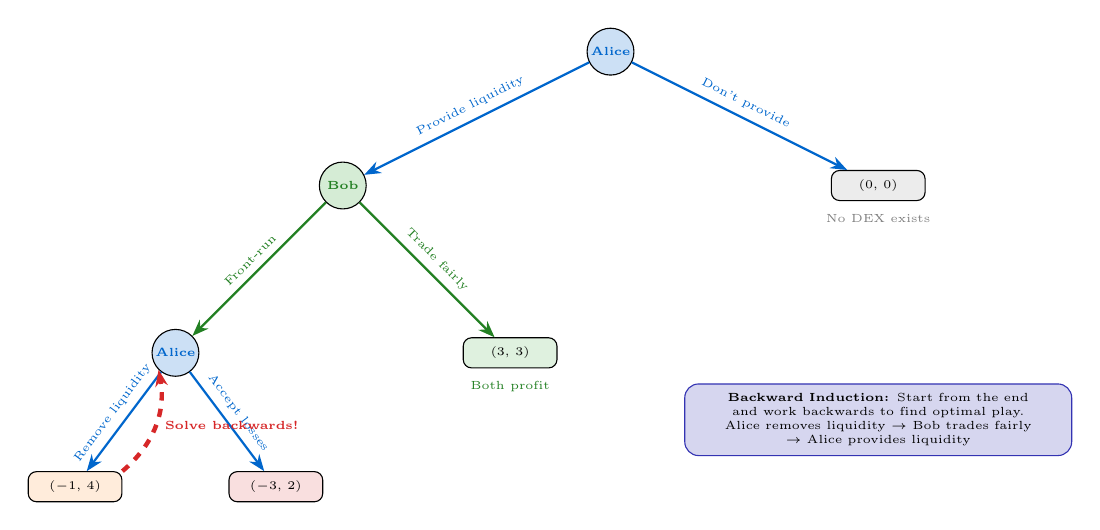
\begin{tikzpicture}[scale=0.85, every node/.style={transform shape}]

% Alice's initial decision
\node[gtdecisionc=mlblue!20, text=mlblue] (a1) at (0,3) {Alice};

% Alice branches
\node[gtdecisionc=mlgreen!20, text=mlgreen!80!black] (b1) at (-4,1) {Bob};
\node[gtpayoff=mlgray!15] (p1) at (4,1) {(0, 0)};

\draw[-{Stealth[length=6pt]}, thick, mlblue] (a1) -- (b1)
      node[midway, above, sloped, font=\tiny] {Provide liquidity};
\draw[-{Stealth[length=6pt]}, thick, mlblue] (a1) -- (p1)
      node[midway, above, sloped, font=\tiny] {Don't provide};
\node[font=\tiny, mlgray] at (4,0.5) {No DEX exists};

% Bob's decision
\node[gtdecisionc=mlblue!20, text=mlblue] (a2) at (-6.5,-1.5) {Alice};
\node[gtpayoff=mlgreen!15] (p2) at (-1.5,-1.5) {(3, 3)};

\draw[-{Stealth[length=6pt]}, thick, mlgreen!80!black] (b1) -- (a2)
      node[midway, above, sloped, font=\tiny] {Front-run};
\draw[-{Stealth[length=6pt]}, thick, mlgreen!80!black] (b1) -- (p2)
      node[midway, above, sloped, font=\tiny] {Trade fairly};
\node[font=\tiny, mlgreen!80!black] at (-1.5,-2.0) {Both profit};

% Alice's response to front-run
\node[gtpayoff=mlorange!15] (p3) at (-8,-3.5) {($-$1, 4)};
\node[gtpayoff=mlred!15] (p4) at (-5,-3.5) {($-$3, 2)};

\draw[-{Stealth[length=6pt]}, thick, mlblue] (a2) -- (p3)
      node[midway, above, sloped, font=\tiny] {Remove liquidity};
\draw[-{Stealth[length=6pt]}, thick, mlblue] (a2) -- (p4)
      node[midway, above, sloped, font=\tiny] {Accept losses};

% Backward induction arrow
\draw[-{Stealth[length=6pt]}, ultra thick, mlred, dashed] (p3.north east) to[bend right=30]
      node[midway, right, font=\tiny\bfseries, text=mlred] {Solve backwards!} (a2.south west);

% Explanation box
\node[draw=mlpurple, fill=mllavender4, rounded corners=5pt, font=\tiny,
      text width=5.5cm, align=center, inner sep=4pt] at (4,-2.5)
      {\textbf{Backward Induction:} Start from the end\\and work backwards to find optimal play.\\Alice removes liquidity $\rightarrow$ Bob trades fairly\\$\rightarrow$ Alice provides liquidity};

\end{tikzpicture}
\end{center}
\bottomnote{Extensive form games show the order of decisions --- solve them by working backwards from the final payoffs.}
\end{frame}

%% ============================================================
%% FRAME 20: REAL CRYPTO GAME THEORY
%% ============================================================
\begin{frame}{Real Crypto Game Theory --- Case Studies}
\vspace{-2mm}
\begin{center}
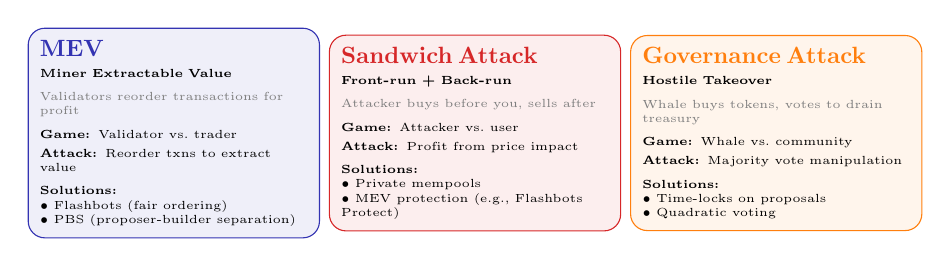
\begin{tikzpicture}[scale=0.85, every node/.style={transform shape}]

% Card 1: MEV
\node[draw=mlpurple, fill=mlpurple!8, rounded corners=6pt,
      text width=4cm, inner sep=5pt, align=left, font=\tiny]
      (card1) at (-4.5,1.0)
      {\textbf{\normalsize\textcolor{mlpurple}{MEV}}\\[3pt]
       \textbf{Miner Extractable Value}\\[4pt]
       \textcolor{mlgray}{Validators reorder transactions for profit}\\[4pt]
       \textbf{Game:} Validator vs.\ trader\\[2pt]
       \textbf{Attack:} Reorder txns to extract value\\[4pt]
       \textbf{Solutions:}\\
       $\bullet$ Flashbots (fair ordering)\\
       $\bullet$ PBS (proposer-builder separation)};

% Card 2: Sandwich
\node[draw=mlred, fill=mlred!8, rounded corners=6pt,
      text width=4cm, inner sep=5pt, align=left, font=\tiny]
      (card2) at (0,1.0)
      {\textbf{\normalsize\textcolor{mlred}{Sandwich Attack}}\\[3pt]
       \textbf{Front-run + Back-run}\\[4pt]
       \textcolor{mlgray}{Attacker buys before you, sells after}\\[4pt]
       \textbf{Game:} Attacker vs.\ user\\[2pt]
       \textbf{Attack:} Profit from price impact\\[4pt]
       \textbf{Solutions:}\\
       $\bullet$ Private mempools\\
       $\bullet$ MEV protection (e.g., Flashbots Protect)};

% Card 3: Governance
\node[draw=mlorange, fill=mlorange!8, rounded corners=6pt,
      text width=4cm, inner sep=5pt, align=left, font=\tiny]
      (card3) at (4.5,1.0)
      {\textbf{\normalsize\textcolor{mlorange}{Governance Attack}}\\[3pt]
       \textbf{Hostile Takeover}\\[4pt]
       \textcolor{mlgray}{Whale buys tokens, votes to drain treasury}\\[4pt]
       \textbf{Game:} Whale vs.\ community\\[2pt]
       \textbf{Attack:} Majority vote manipulation\\[4pt]
       \textbf{Solutions:}\\
       $\bullet$ Time-locks on proposals\\
       $\bullet$ Quadratic voting};

\end{tikzpicture}
\end{center}
\bottomnote{These are real game-theory attacks happening on-chain today --- understanding them is essential for building secure DeFi protocols.}
\end{frame}

%% ============================================================
%% FRAME 21: YOUR GAME THEORY TOOLKIT
%% ============================================================
\begin{frame}{Your Game Theory Toolkit}
\vspace{-2mm}
\begin{center}
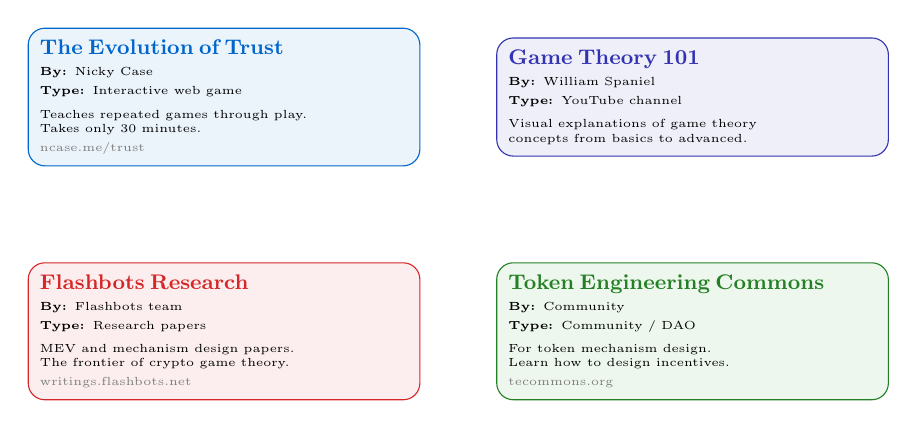
\begin{tikzpicture}[scale=0.85, every node/.style={transform shape}]

% Card 1
\node[draw=mlblue, fill=mlblue!8, rounded corners=6pt,
      text width=5.5cm, inner sep=5pt, align=left, font=\tiny]
      (r1) at (-3.5,2.0)
      {\textbf{\small\textcolor{mlblue}{The Evolution of Trust}}\\[3pt]
       \textbf{By:} Nicky Case\\[2pt]
       \textbf{Type:} Interactive web game\\[4pt]
       Teaches repeated games through play.\\
       Takes only 30 minutes.\\[2pt]
       \textcolor{mlgray}{ncase.me/trust}};

% Card 2
\node[draw=mlpurple, fill=mlpurple!8, rounded corners=6pt,
      text width=5.5cm, inner sep=5pt, align=left, font=\tiny]
      (r2) at (3.5,2.0)
      {\textbf{\small\textcolor{mlpurple}{Game Theory 101}}\\[3pt]
       \textbf{By:} William Spaniel\\[2pt]
       \textbf{Type:} YouTube channel\\[4pt]
       Visual explanations of game theory\\concepts from basics to advanced.};

% Card 3
\node[draw=mlred, fill=mlred!8, rounded corners=6pt,
      text width=5.5cm, inner sep=5pt, align=left, font=\tiny]
      (r3) at (-3.5,-1.5)
      {\textbf{\small\textcolor{mlred}{Flashbots Research}}\\[3pt]
       \textbf{By:} Flashbots team\\[2pt]
       \textbf{Type:} Research papers\\[4pt]
       MEV and mechanism design papers.\\
       The frontier of crypto game theory.\\[2pt]
       \textcolor{mlgray}{writings.flashbots.net}};

% Card 4
\node[draw=mlgreen!80!black, fill=mlgreen!8, rounded corners=6pt,
      text width=5.5cm, inner sep=5pt, align=left, font=\tiny]
      (r4) at (3.5,-1.5)
      {\textbf{\small\textcolor{mlgreen!80!black}{Token Engineering Commons}}\\[3pt]
       \textbf{By:} Community\\[2pt]
       \textbf{Type:} Community / DAO\\[4pt]
       For token mechanism design.\\
       Learn how to design incentives.\\[2pt]
       \textcolor{mlgray}{tecommons.org}};

\end{tikzpicture}
\end{center}
\bottomnote{Start with `The Evolution of Trust' --- it teaches repeated games through play and takes only 30 minutes.}
\end{frame}

\end{document}
